% interactcadsample.tex
% v1.03 - April 2017

\documentclass[]{interact}

\usepackage{epstopdf}% To incorporate .eps illustrations using PDFLaTeX, etc.
\usepackage{subfigure}% Support for small, `sub' figures and tables
%\usepackage[nolists,tablesfirst]{endfloat}% To `separate' figures and tables from text if required

\usepackage{natbib}% Citation support using natbib.sty
\bibpunct[, ]{(}{)}{;}{a}{}{,}% Citation support using natbib.sty
\renewcommand\bibfont{\fontsize{10}{12}\selectfont}% Bibliography support using natbib.sty

\theoremstyle{plain}% Theorem-like structures provided by amsthm.sty
\newtheorem{theorem}{Theorem}[section]
\newtheorem{lemma}[theorem]{Lemma}
\newtheorem{corollary}[theorem]{Corollary}
\newtheorem{proposition}[theorem]{Proposition}

\theoremstyle{definition}
\newtheorem{definition}[theorem]{Definition}
\newtheorem{example}[theorem]{Example}

\theoremstyle{remark}
\newtheorem{remark}{Remark}
\newtheorem{notation}{Notation}

\begin{document}

\articletype{ARTICLE DRAFT}

\title{Modelling and optimization of ship's fuel consumption using Random Forest Regression (RFR)}

\author{
\name{Muhammad Fakhruriza Pradana\textsuperscript{a,b}\thanks{Muhammad Fakhruriza Pradana. Email: mfakhruriza@untirta.ac.id}, Hibatul Wafi\textsuperscript{b}, Bernd Noche\textsuperscript{b}}
\affil{\textsuperscript{a}Department of Civil Engineering, University of Sultan Ageng Tirtayasa, Cilegon, Indonesia ; \textsuperscript{b}Institute of Transport Systems and Logistics, University of Duisburg-Essen, Duisburg, Germany}
}

\maketitle

\begin{abstract}
Efforts to model energy-efficient operation of shipping operations using machine-learning methods have emerged due to volatile bunker fuel prices and stringent environmental regulations. It is widely regarded that ship speed is one of the most influential factors impacting ships' fuel oil consumption and as such, accurate modelling of ship speed is paramount to ensure the accuracy of subsequent FOC prediction.

This study proposes an intuitive data-driven modelling approach, integrating Automatic Identification System and weather data for modelling of ship states and environmental conditions' impact on FOC. Grey Box Modelling approach divides the speed and FOC prediction into stages, the first stage involves the prediction of speed over ground using Random Forest Regressor. Consequently, the FOC prediction based on predicted speed employs the empirical formula by Holtrop-Mennen, maintaining adherence with established vessel knowledge.
  
In the presented case study, optimised SOG prediction achieves $3.94\%$ mean absolute percentage error (MAPE) and $93.41\%$ $R^2$ score. Subsequent FOC prediction from estimated speed yields $86.57\%$ $R^2$ and $12.06\%$ MAPE. The results affirm the proposed approach's viability in predicting energy-efficient ship operations.
\end{abstract}

\begin{keywords}
Energy-efficient operation; Random Forest Regression; Ship speed prediction; Fuel consumption prediction; Grey Box Model; AIS 
\end{keywords}


\section{Introduction}

The marine industry is actively researching efficient ship operation due to rising fuel prices and stricter environmental rules. Fuel costs, known as "bunkers," comprise over 50\% of voyage expenses and up to 75\% of total operating costs, impacting profitability \citep{Bialystocki.2016}. Energy-efficient practices reduce costs and greenhouse gas emissions, crucial with shipping contributing 2.51\% of global emissions \citep{IMO.2020}. This mutual motivation aligns economic benefits with environmental compliance. Stakeholders seek solutions to energy-efficient operation by considering technical and operational approaches. Technical solutions require costly structural and power system alterations \citep{Yan.2021,Li.2022}, prompting interest in the cost-effective, optimisation of operational measures.

Significant emphasis is given in this study on optimisation of ship speed due to its substantial impact on fuel consumption which is caused by a third-order non-linear correlation between fuel consumption and ship speed \citep{Wang.2012,Du.2019}. However, the process of optimising the speed prediction model is intricate, appropriate features must be considered as the ship speed is influenced by factors like vessel performance and weather conditions.

Fuel consumption models based on historical data and ship parameters lack robustness and sensitivity to noise. To address this, recent research employs data-driven techniques, like machine learning (ML), for ship speed and fuel consumption prediction. ML models showcase strong generalisation capabilities and low prediction errors, although some experts are reluctant to accept the generated models by the machine learning approach due to their complexity, unintuitiveness, and potential violation of vessel physics. The success of data-driven models is also highly dependent on data quality and quantity \citep{Yan.2021,Gkerekos.2019}. Given volatile fuel prices, developing an accurate Fuel Oil Consumption (FOC) prediction model is valuable for maritime stakeholders. This aids in timely economic decisions without violating environmental regulations.

The following Research Questions (RQs) could be raised during the development of the model :

\begin{itemize}
    \item \textbf{RQ1}: What are the steps that should be taken to optimise the predictive performance of the model?
    \item \textbf{RQ2}: Is it feasible to fuse AIS data and meteorological data to accurately predict the ship's SOG and subsequently FOC of the ship?
    \item \textbf{RQ3}: Which approximations and empirical equations are suitable to estimate the resistance forces required to estimate the power required by the ship? 
\end{itemize} 

The following research boundaries are set throughout this thesis:

\begin{itemize}
    \item The weather information and AIS data are assumed to be true. Any uncertainties from AIS data and weather data are neglected. 
    \item The focus of this work is a detailed study of the performance and possible optimisation configuration of Random Forest (RF) as predictors for SOG. As such, an exhaustive comparison study between different types of machine learning models will not be performed.
    \item In the case study, the approximation for incomplete ship parameters and dimensions is based on a similar type of ship with nearly identical dimensions. 
\end{itemize}

The Grey Box (GB) modelling approach using the fusion of AIS data and weather data provides the following contributions : 

\begin{itemize}
    \item Economical and independent data source.
    \item Robust modelling approach that requires minimal data pre-processing and minimal model configuration.
    \item Comprehensible model that adheres to physical principles and hydrodynamic laws of the vessel.  
\end{itemize} 


\section{Literature Review}\label{sec:literature_review}

\subsection{Modelling Approach for Ship Operation}\label{sec:modelling_type}

\citet{haranen2016white} and \citet{Coraddu.2017} categorised fuel consumption prediction models into three strategies:

\textbf{White Box Models (WBM)}: Built on prior mechanistic knowledge and physical principles of a vessel's system, including its structure, design parameters, and propulsion configuration.

\textbf{Black Box Models (BBM)}: Data-driven and developed using data from different sailing journeys and historical observations. The Machine Learning (ML) modelling approach focuses on the prediction of bunker consumption at different points in time.

\textbf{Grey Box Models (GBM)}: A fusion of WBM and BBM, resulting in a single model that considers both \emph{a priori} knowledge of the vessel and historical sailing data, This method aims to complement the performance of WBM and BBM.

Each strategy has strengths and weaknesses. WBM is transparent and comprehensible, rooted in physics and hydrodynamics, but lacks adaptability and generalisation due to its deterministic nature and dependence on prior knowledge. BBM excels in fitting and predicting data but lacks vessel-specific knowledge and can be complex. To achieve good prediction, it requires an abundance of data quantity and good data quality \citep{Halevy.2009}. GBM mitigates these limitations by combining mechanistic understanding with predictive capabilities.

The modelling of FOC using GBM requires both components of WBM and BBM. For the BBM modelling part using ML approach, For black-box modelling using ML techniques, it is crucial to have sufficient high-quality data for accurate training \citep{Halevy.2009}. \citet{Yan.2021} categorise the data sources for FOC modelling as follows:

\subsection{Automatic Identification System (AIS) data}\label{sec:ais_theo_j}

Besides its intended role as a collision avoidance system, Automatic Identification System (AIS) data finds potential in ship behaviour analysis and environmental assessment. The International Maritime Organization (IMO) utilized AIS data to study Greenhouse Gas (GHG) emissions, estimating global shipping emissions \citep{IMO.2020,T.W.P.Smith.2015}. \citet{Rakke.2016} introduced ECAIS as a methodology to compute ship emissions from AIS-derived fuel consumption data using Holtrop-Mennen and literature-based approximations. The study by \citet{Kim.2020b} used AIS data, ship information, and environmental data for estimating Energy Efficiency Operational Indicator (EEOI). The use of AIS data in research aims for data independence, reducing reliance on commercial databases.

It is also stated by \citet{Yang.2019} that AIS data can be combined with data from other databases to provide additional information such as:

\begin{itemize}
    \setlength\itemsep{0em}
    \item Port-to-port average speed: the voyage time can be calculated from the time stamps reported by AIS data; the voyage distance can be found from corresponding navigation distance tables.
    \item Cargo weight which can be estimated from draught and ship size.
    \item Technical ship specification from fleet database which can be derived from IMO number.
    \item Port-to-port bunker consumption which can be estimated based on the speed, technical ship specification and distance between two ports.
\end{itemize}

\subsection{Predictive performance of tree based models}\label{sec:perf_tree_litreview}

Tree-based model is a supervised, highly interpretable BBM modelling approach using machine learning approach which is adept in classification and regression tasks. The model is inherently resistant to multicollinearity problems \citep{Yan.2021}.  Several literature studies reveal its advantages and performance superiority. \citet{Soner.2018} employed ferry data to predict FOC using tree-based models including bagging, random forest (RF), and bootstrap. RF achieved $43.5$ L/h RMSE for fuel consumption, outperforming Artificial Neural Network (ANN) model employed by \citet{Petersen.2012}.

\citet{Yan.2020} predicted FOC for a dry bulk ship's voyage using RF. The model incorporated sailing speed, cargo weight, and meteorological conditions, it is able to attain mean absolute percentage error (MAPE) of $7.91\%$ and the RF model outperformed decision tree, ANN, LASSO, and SVR. \citet{Gkerekos.2019} compared ML models to predict daily FOC, RF model achieved $89\%$ and $96\%$ $R^2$ scores with noon data and ADLM system data, respectively. \citet{Li.2022} fused meteorological, voyage, and AIS data to explore the effect of data on ML models for FOC prediction. Tree-based models (bagging and boosting ensembles) including ETR, RFR, AB, GB, XG, and LB were recommended for energy-efficient operation modelling, with RFR particularly displaying the best robustness among the presented ML models in the study. \citet{Abebe.2020} predicted ship speed over ground (SOG) using AIS and weather data. The RF model achieved $98\%$ $R^2$ score and $0.25$ knots RMSE.

WBMs for predicting FOC utilize physics and hydrodynamic laws to compute the vessel's resistance, encompassing calm water resistance and additional effects like wind and waves. Then the engine power can be subsequently estimated at a specific speed, facilitating FOC calculation \citep{haranen2016white}. Holtrop-Mennen power estimation method \citet{Holtrop.1984}, is applicable in a wide range \citep{Rakke.2016,Kim.2020b}. \citet{Rakke.2016} utilized AIS data and mechanical information to estimate engine power using Holtrop-Mennen, achieving about $5\%$ model testing error for FOC and GHG emissions estimation. Similarly, \citet{Kim.2020b} estimated Energy Efficiency Operational Index (EEOI) through Holtrop-Mennen-based engine power estimation, enabled by AIS data and weather information.

\section{Methodology}\label{sec:big_methodology}

This chapter covers the methodology used to construct the grey box model (GBM). The grey box approach employed in this study is categorised as sequential GBM, which entails a two-stage development process. The initial stage focuses on machine learning modelling using tree-based models. The modelling is carried out using Python in conjunction with \texttt{Scikit-Learn} \citep{FabianPedregosa.2011}. 
\begin{figure}
  \centering
      
\includegraphics[width=.75\textwidth]{00_figures/flowmethod_BBM_alt.png}
      \caption{Scheme of proposed BBM methodology}
      \label{fig:flowchart_BBM}
\end{figure}

The second stage of the modelling process revolves around the power estimation method \citep{Holtrop.1984}. This involves an initial conversion of SOG to STW for estimation of encountered resistance during the voyage, this then facilitates the estimation of the required power i.e. the energy required to propel the ship.

\begin{figure}
  \centering
      
\includegraphics[width=.75\textwidth]{00_figures/flowmethod_WBM.png}
      \caption{Scheme of proposed BBM methodology}
      \label{fig:flowchart_GBM}
\end{figure}

\subsection{Data Acquisition}\label{sec:data_acquisition}

The data is collected from a ferry serving between the ports of K{\o}ge, R{\o}nne, Ystad, and Sassnitz. The trip duration between K{\o}ge and R{\o}nne is approximately 5 hours and 30 minutes, while the voyage between Rønne and Sassnitz takes around 3 hours and 20 minutes. The Danish Maritime Authority's (DMA) T-AIS system tracks the journey. Weather data along the ferry's route is sourced from ECMWF, providing information on wind, waves, and seawater temperature. This data has a temporal resolution of 1 hour and a spatial granularity of 0.25° (longitude) x 0.25° (latitude). Current information, obtained from CMEMS, is available at a temporal resolution of 3 hours and a spatial granularity of 0.25° (longitude) x 0.25° (latitude). The resulting combined dataset maintains a temporal resolution of 1 hour. To address the temporal resolution disparity between CMEMS and ECMWF data, the weather information is synchronized. This synchronization ensures that the wind, waves, seawater temperature, and sea current data are aligned with the same weather grid and maintain consistent temporal resolutions.

\begin{figure}
  \begin{minipage}{0.55\linewidth} % Adjust the width as needed
    \footnotesize
    \centering
    \begin{tabular}{l r}
        \hline
        IMO & 9812107 \\
        Type \& Service & Passenger ferry \\
        $L_{OA}$ & 158.00 m\\
        $L_{WL}$ & 144.80 m\\
        $B$ (moulded) & 24.5 m\\
        $T_{DESIGN}$ & 5.70 m\\
        $T_{MAX}$ & 5.85 m \\ 
        Gross Tonnage (GT) & 18,009 \\
        Deadweight (dwt) & 4,830 t \\
        Main Engines & Wärtsillä 8V31 2 x 4,880 kW \\
        SFOC & 169.4 g/kWh \\
        Service Speed & 17.7 knots \\
        Bow Thrusters & 2 x 1500 kW \\
        \hline
    \end{tabular}
    \caption{Particular of M/S Hammershus}
    \label{tbl:Hammershus_Data}
  \end{minipage}
  \hspace{0.01\linewidth}
%   \hfill
  \begin{minipage}{0.43\linewidth} % Adjust the width as needed
    \centering
    % \vspace*{0.1cm}
    \includegraphics[width=\linewidth]{00_figures/Bornholmerfærgen_route_map.png} % Replace example-image.jpg with your picture file name
    \caption{Journey of the ferry}
    \label{fig:Hammershus_journey_map}
  \end{minipage}
\end{figure}

\begin{figure}
  \centering
      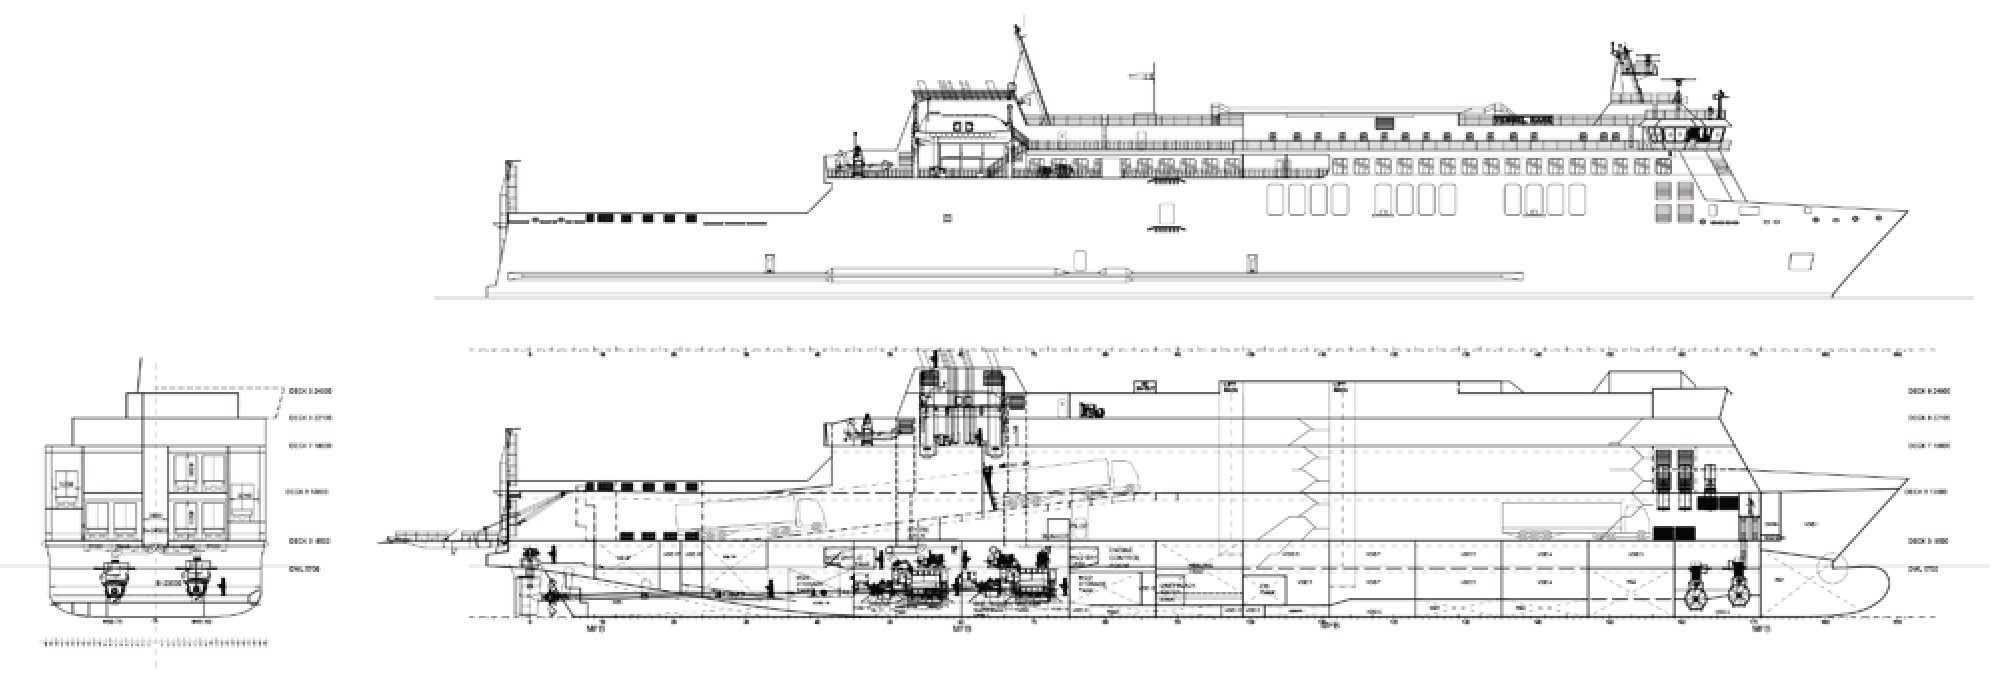
\includegraphics[width=.75\textwidth]{00_figures/Hammershus_Pict.jpg}
      \caption{Schematics of M/S Hammershus}
      \label{fig:Hammershus_Pict}
\end{figure}

\subsection{Data Pre-Processing}\label{sec:data_prep}

This section outlines the data preprocessing steps, including data cleaning to identify anomalies and the handling of missing values. threshold application to the Speed Over Ground (SOG) and feature selection that is based on domain knowledge, ensuring alignment with vessel characteristics. The procedures are performed to ensure that the dataset is in the state required for modelling. 

\subsubsection{Data Cleaning}\label{sec:data_cleaning}

Analysis of the data points indicated an incomplete representation of the voyage between R{\o}nne and Sassnitz due to limitations in the T-AIS system's coverage. Therefore, a latitude threshold of 55.04° N is implemented, excluding the voyage segment between Sassnitz and R{\o}nne. To ensure that the dataset accurately captures the ship's operational conditions under steady state, a threshold is applied to the SOG. The change in SOG can originate from changing sea conditions or intentional speed adjustments during port arrivals and departures. Therefore, data points with SOG below 5 knots, indicative of manoeuvring or stationary activities, are removed from the dataset \citep{Abebe.2020, Yan.2020}. As a result of this filtering process, the dataset size notably reduces from 7,453 data points to 3,828 data points. This reduction highlights that approximately half of the initial data points correspond to periods when the ship was stationary or engaged in low-speed manoeuvres.

Missing and \texttt{NaN} values are imputed using the \texttt{KNNImputer} feature from \texttt{Scikit-Learn}. This step is essential as the modelling package provided by \texttt{Scikit-Learn} cannot handle instances with missing values. The choice of using a k-nearest neighbour imputation strategy is appropriate, as it aims to capture the weather conditions within the vicinity of the missing values.

\subsubsection{Feature Selection}\label{sec:feature_select}

To select appropriate features for the model, feature correlation is analyzed. Feature selection aims to simplify the model and reduce computational costs during training. The High Correlation Filter, proposed by \citet{Abebe.2020}, is used. It treats feature pairs with correlation coefficients above 0.7 as a single entity. However, feature selection here is primarily guided by physical reasoning, prioritizing physical principles over statistics.

Features from AIS data such as \emph{time, latitude, longitude, width,} and \emph{length} are excluded, as they only represent ship location and constant dimensions. Features from weather data, such as \emph{combined wind wave swell height, swell height, maximum wave height,} and \emph{wind wave height,} are interconnected by physical relationships. The combined wind wave swell height corresponds to significant wave height $H_{1/3}$. Additionally, significant wave height can be used to identify whether the sea is dominated by swell or wind-generated waves \citep{BitnerGregersen.2005}. Hence, it is evident that retaining the significant wave height is essential for the model, given that various wave properties can be deduced from it. 

In a statistical context, heading and COG exhibit significant correlations. However, both features are retained due to their representation of distinct ship parameters. Course Over Ground (COG) signifies the ship's course heading while heading signifies the ship's actual heading at a specific time point. A similar rationale applies to the relationship between air temperature above the ocean and sea surface temperature. Air temperature above oceans represents wind temperature, whereas sea surface temperature reflects the temperature of the water surface.

\begin{figure}[h!]
  \centering
  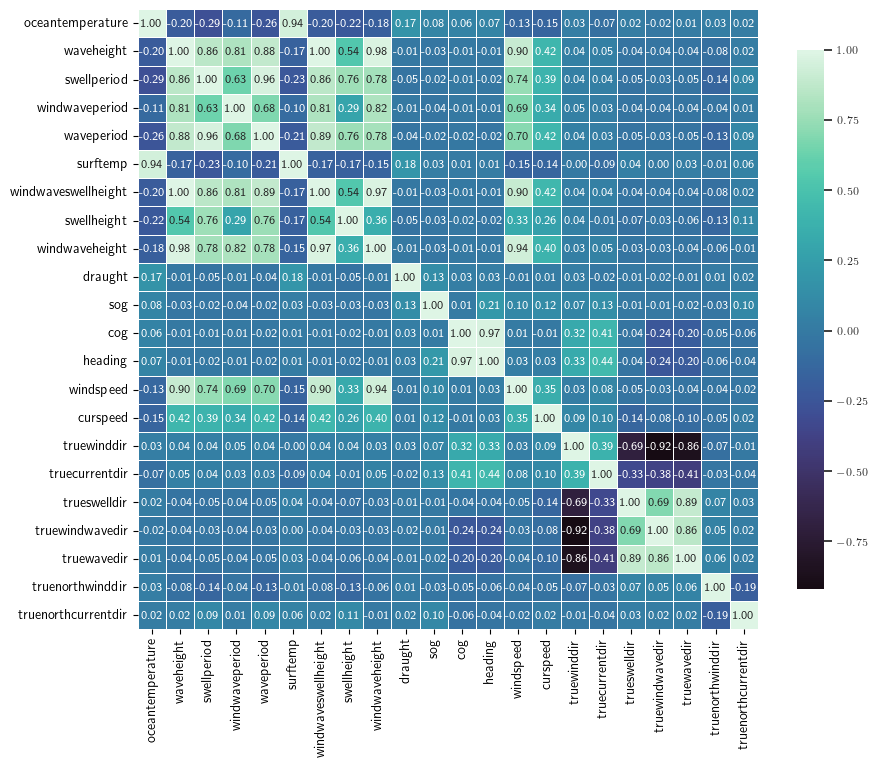
\includegraphics[width=.8\linewidth,height=.8\textheight,keepaspectratio]{00_figures/heatmap_corr_ovr.png}
  \caption{Correlation Heat Map}
  \label{fig:heatmap_ovr}
\end{figure}


\begin{table}
\tbl{Structure of training dataset}
  % \footnotesize
  % \centering
  % \resizebox {\textwidth}{!}
  {\begin{tabular}{ p{8cm}c }
  \hline
  \multicolumn{2}{l}{\textbf{Training Label}}\\
  \hline
  SOG [Knots] & {\tt sog} \\
  \hline
  \multicolumn{2}{l}{\textbf{Training Features}}\\
  \hline
  COG [°] & {\tt cog}  \\
  Heading [°] & {\tt heading}  \\
  Draught [m] & {\tt draught} \\
  Wind Speed [m/s] & {\tt windspeed} \\
  Air Temperature Above Oceans [K] & {\tt oceantemperature} \\
  % Maximum Wave Height [m] & {\tt waveheight} \\
  Wave Period [s] & {\tt waveperiod}\\
  Sea Surface Temperature [K] & {\tt surftemp}\\
  Combined Wind Wave Swell Height [m] &  {\tt windwaveswellheight} \\
  Current Speed [m/s] & {\tt curspeed} \\
  True Wind Direction [°] & {\tt truewinddir}  \\
  True Current Direction [°] & {\tt truecurrentdir} \\
  True Wave Direction [°] & {\tt truewavedir} \\
  \hline
  \end{tabular}}
% \caption{Structure of training dataset}
\label{tbl:struct_train_final}
\end{table}

\subsection{Modelling methodologies}\label{sec:tree_model_development}

\subsubsection{Decision Tree (DT) Regressor}\label{sec:dt_theo_j}

The Decision Tree operates by employing nested {\tt if-then} statements based on predefined rules, resulting in a partitioned data space. This process can also be visualized as a binary tree, enhancing interpretability by representing diverse input responses within a single tree \citet{Kuhn.2013, Hastie.2009}.

A Decision Tree encompasses distinct nodes: the \textbf{\emph{Root node}} represents the top-level node; \textbf{\emph{Leaf nodes}} (or terminal nodes) yield final prediction outcomes; and \textbf{\emph{Internal nodes}} lie between the root and leaf nodes. The procedure of dividing a node into subsequent nodes is termed \textbf{\emph{splitting}}, where the original node is the \textbf{\emph{parent node}} and the resultant nodes are \textbf{\emph{child nodes}}. In regression tasks, tree growth is often controlled by Mean Square Error (MSE), guided by the Classification and Regression Tree (CART) algorithm, The notation $J(\text{k},\text{t}_k)$ represents the cost function that needs to be minimised.

\begin{equation}\label{eqn:sse}
  \text{MSE}_{\text{s}_i} = \frac{1}{n_{\text{s}_i}}\text{SSE}_{\text{s}_i} \quad \textbf{where} \quad i = (1,2)   
\end{equation}
\begin{equation}\label{eqn:costfun}
  J(\text{k},\text{t}_k) = \frac{1}{n_{\text{s}_1}}\text{SSE}_{\text{s}_1} + \frac{1}{n_{\text{s}_2}}\text{SSE}_{\text{s}_2}
  \begin{cases}
      \text{SSE}_{\text{s}_i} = \sum\limits_{i \in \text{s}_i}(\hat{y}_{\text{s}_i} - y_{\text{s}_i} )^2 \\
      \hat{y}_{\text{s}_i} = \frac{1}{n_{\text{s}_i}}\sum\limits_{i\in \text{s}_i} y
  \end{cases}  
\end{equation}

The process of tree growth stops until either the number of samples for splitting reaches a predefined threshold or when no further split can be found which reduces the MSE. The decisions from optimal splits are visualised through a binary tree representation, enhancing the interpretability and ease of implementation. The inherent logic structure of decision trees enables them to handle diverse data types without extensive preprocessing, including sparse, skewed, continuous, and categorical data. Decision trees also inherently perform feature selection, which is a valuable aspect in modelling \citep{Kuhn.2013}.

However, an unconstrained single decision tree is prone to overfitting due to its tendency to closely match the training data. This model's instability can lead to substantial changes in its structure when the data is altered, resulting in a completely different interpretation of splits \citep{Hastie.2009, Kuhn.2013}. To mitigate overfitting, it becomes essential to regularise the decision tree's growth during training. The following parameters control the growth of a single decision tree : 

\begin{itemize}
  \item \texttt{max\_depth}: This hyperparameter is defined as the count of nodes along a path from the root node to its parent node. The default parameter allows full unpruned growth of the tree.
  \item \texttt{min\_samples\_leaf}: This hyperparameter controls the number of samples required to be at the leaf node, where the split point will be considered if the leaf contains at least {\tt min\_samples\_leaf=n} training samples in each left and right branch.
  \item \texttt{min\_samples\_split}: This hyperparameter controls the minimum number of samples i.e. data points required to split a node.    
\end{itemize}

\subsubsection{Random Forest (RF) Regressor}\label{sec:rf_theo_j}

Ensemble learning offers a solution to enhance the performance of Decision Tree (DT) regressors. This concept involves combining the strengths of multiple simpler base models \citep{Hastie.2009}. One prominent ensemble method is the \textbf{\emph{Random Forest}}, introduced by \citet{Breiman.2001}, which involves creating bootstrap samples, randomly selecting splitting features, and aggregating predictions. This approach combines various learning algorithms, referred to as weak learners, with each corresponding to an individual decision tree in the Random Forest. Random forest uses the Bagging (\emph{bootstrap aggregating}) strategy, where it trains each tree using bootstrap samples, where instances from the training set are randomly selected with replacement.

To further improve bagging, reducing the correlation between trees is applied. This involves introducing randomness during tree construction. Random split selection, as introduced by \citet{Dietterich.2000}, involves selecting a feature from a random subset for each split. This, coupled with the inherent instability of a single decision tree, addresses overfitting and the lack of robustness of DTR. The Random Forest methodology addresses these issues by creating an ensemble of independent, strong learners, resulting in reduced variance and robustness against noisy data \citep{Breiman.2001}. While losing some interpretability compared to basic tree-based models, the impact of each feature in the ensemble can still be quantified \citep{Kuhn.2013}. Random Forest performs better with larger sample sizes, and extensive parameter tuning is often unnecessary for good prediction results \citep{Kuhn.2013, Hastie.2009}.

In addition to the hyperparameters used to fine-tune the decision tree, the RF model provides additional hyperparameters to control the growth of the tree:

\begin{itemize}
  \item \texttt{max\_features}: This hyperparameter controls the number of features to be considered when looking for the best split. The default parameter considers all features during training.
  \item \texttt{n\_estimators}: This hyperparameter controls the number of trees i.e. predictors in a forest.
\end{itemize}

\subsubsection{Model Hyperparameter Optimisation}\label{sec:hpo_opti_J}

\texttt{Scikit-Learn} provides both the {\tt GridSearchCV} and {\tt RandomizedSearchCV} methods to assist in the search for optimal hyperparameters. Both approaches share a similar principle: the specified hyperparameters and their corresponding value ranges are evaluated through cross-validation to determine the best combination. The distinction between {\tt GridSearchCV} and {\tt RandomizedSearchCV} lies in how they search for the best hyperparameter values:

\begin{itemize}
  \item {\tt GridSearchCV}: This method constructs a grid comprising all possible combinations of hyperparameter values within the specified ranges. It exhaustively explores this grid to find the best combination.
  \item {\tt RandomizedSearchCV}: Randomly samples hyperparameter values from the specified ranges. It offers more control over computational resources by allowing the specification of the number of iterations. This method often produces accurate results and is computationally more efficient than {\tt GridSearchCV} \citep{J.Bergstra.2012}.
\end{itemize}

Due to the computational limitation posed by exhaustive grid search, the {\tt RandomizedSearchCV} approach will be adopted to identify optimal hyperparameters. 

\subsubsection{Holtrop-Mennen Method}\label{sec:Holtrop_mennen_j}

A ship's bunker fuel consumption in actual operating conditions is affected by several factors including the operating parameter of the ship's engine, propeller efficiency, and encountered resistance by the ship. Furthermore, a ship's propulsion power is correlated to the sailing speed (SOG) and meteorological conditions \citep{XiaoLang.2020}. Therefore, in addition to the calm water resistance $R_{CALM}$, the additional resistance caused by wind $R_{AA}$ and wave $R_{AW}$ should be considered to estimate the total resistance of the ship $R_{TOTAL}$. The power needed to propel a ship forward at a given ship STW $v_S$, to overcome $R_{TOTAL}$ is defined as \textbf{effective power $P_e$}:

\begin{equation}\label{eqn:R_tot}
    R_{TOTAL} = R_{CALM} + R_{AW} + R_{AA} 
\end{equation}

\begin{equation}\label{eqn:P_e}
    P_e = R_{TOTAL}\cdot v_{S}
\end{equation}

The effective power $P_e$ is transmitted through the shaft connected to the main engine of the ship which generates power to rotate the propeller of the ship, which is termed as \textbf{brake power of the engine, $P_b$}. The brake power can be calculated through effective power by considering the \textbf{shaft efficiency $\eta_s$, hull efficiency $\eta_h$, relative rotative efficiency $\eta_r$ and open water efficiency $\eta_o$}:

\begin{equation}\label{eqn:P_b}
    P_b = \frac{P_e}{\eta_s\cdot\eta_h\cdot\eta_r\cdot\eta_o}
\end{equation}

The bunker fuel consumption can then be calculated by multiplying the brake power $P_b$ with the Specific Fuel Oil Consumption (SFOC) and the operation time $\tau_{OP}$:

\begin{equation}\label{eqn:FOC}
    FOC = P_b\cdot SFOC\cdot \tau_{OP} 
\end{equation}

Since the speed that is represented in AIS data is SOG, $v_G$, given the current speed $v_C$ and the current direction with respect to true north $\gamma$, the conversion to speed through water STW, $v_S$ is done by the following equations \citep{Kim.2020b}:

\begin{equation}\label{eqn:sogx}
  v_{\text{G}}^x = v_{\text{G}}\cdot\sin(\alpha)   
\end{equation}
\begin{equation}\label{eqn:sogy}
  v_{\text{G}}^y = v_{\text{G}}\cdot\cos(\alpha)   
\end{equation} 
\begin{equation}\label{eqn:vcurrx}
   v_{\text{C}}^x = v_{\text{C}}\cdot\sin(\gamma)   
\end{equation}
\begin{equation}\label{eqn:vcurry}
  v_{\text{C}}^y = v_{\text{C}}\cdot\cos(\gamma)   
\end{equation}

\begin{equation}\label{eqn:stwx}
  v_{\text{S}}^x = v_{\text{G}}^x - v_{\text{C}}^x    
\end{equation}
\begin{equation}\label{eqn:stwy}
  v_{\text{S}}^y = v_{\text{G}}^y - v_{\text{C}}^y      
\end{equation}
\begin{equation}\label{eqn:stwabs}
  v_{\text{S}} = \sqrt{(v_{\text{S}}^x)^2 + (v_{\text{S}}^y)^2} 
\end{equation}

Holtrop-Mennen method has a wide applicability range and it is the only method that adopted the use of the ITTC form factor $k$. The resistances in this method are calculated as dimensional force. Furthermore, the method also gives estimates of hull-propeller interaction, thrust deduction, full-scale wake fraction and relative rotative efficiency \citep{Birk.2019}. For the calculation of the total resistance, the following equations based on the study by \citet{Holtrop.1978,Holtrop.1982,Holtrop.1984}:

\begin{equation}\label{eqn:R_calm}
  R_{CALM} = R_F(1+k_1) + R_{APP} + R_W + R_B + R_{TR} + R_A
\end{equation}

\textbf{$R_F$} is calculated using the ITTC-1957 frictional resistance correlation line $C_F$ as the basis of a representation of a resistance plate with a wetted surface area $S$ of bare hull. The frictional coefficient $C_F$ can be calculated through the Reynold number $Re$ for a given ship speed $v_{S}$ and kinematic viscosity $\nu$: 

\begin{equation}\label{eqn:R_f}
  R_F = \frac{1}{2}\rho v_{S}^2 S C_F 
\end{equation}

An appendage is defined as the addition(s) to the main part or main structure of a vessel \citep{Molland.2011}. Examples of appendages include rudders, shaft brackets, skeg and bilge keels. The form factors associated with these appendages are denoted as $k_{2_i}$. In practice, reasonable estimates can be made based on these form factors, as model tests are not the most suitable method for accurately quantifying appendage resistance. Furthermore, the effects of appendages are typically considered as a whole and not as individual units \citep{Birk.2019}.\\

\begin{equation}\label{eqn:R_app}
  R_{APP} = \frac{1}{2}\rho v_S^2 (1+k_{2_i})_{eq} C_F \sum_i S_{APP_i} + \sum R_{TH}
\end{equation}

If bow thruster is present, the resistance due to the bow thruster tunnel $R_{TH}$ can be obtained through:

\begin{equation}
  \label{eqn:R_th}
  R_{TH} = \rho v_S^2  d_{TH}^2 C_{D_{TH}}
\end{equation}

The coefficient $C_{D_{TH}}$ defines the drag coefficient for the tunnel, and it ranges between $0.003$ and $0.012$.\\

The estimation of wave resistance $R_W$ is dependent on Froude number $Fr$. And it can be obtained through Equation \ref{eqn:R_w_low}. To obtain the formulae to compute the constants, consider the literature work by \citet{Holtrop.1978,Holtrop.1982,Holtrop.1984} and \citet{Birk.2019}.

\begin{equation}\label{eqn:R_w_low}
  R_{W_a}(Fr) = c_1 c_2 c_5 \rho g V  \exp \biggl[ m_1 Fr^d + m_4 \cos(\lambda Fr ^{-2}) \biggr]
\end{equation}

The approximation of the resistance due to bulbous bow $R_B$ can be obtained through the immersion Froude number $F_{r_i}$ for the bulbous bow and the constant $P_B$ which is a measure of the emergence of the bow: 

\begin{equation}
  \label{eqn:Rbulb}
  R_B = 0.11 \rho g (\sqrt{A_{BT}})^3 \frac{Fr_{i}^3}{1+Fr_{i}^2}e^{(-3.0P_B^-2)}
\end{equation}

The term transom refers to the flat section located at the stern of the ship. When the transom becomes immersed in water, it leads to pressure loss, resulting in resistance. This resistance is denoted by the term $R_{TR}$ and is associated with an immersed transom area $A_T > 0$. The transom resistance can be described as a function of the depth Froude number $Fr_{T}$:

\begin{equation}
  \label{eqn:Fr_t}
  Fr_T = \frac{v_S}{\sqrt{\frac{2gA_T}{(B+BC_{WP})}}}
\end{equation}

The expression $A_T/(B+BC_{WP})$ is a measure for the average draught of the transom. When the average draught is smaller than the speed, there will be clean separation of the flow at transom edge and the resistance due to transom vanishes. Immersion resistance $R_{TR}$ is considered if $Fr_{T} > 5$

\begin{equation}
  \label{eqn:R_transom}
  R_{TR} = \frac{1}{2}\rho v_S^2 A_T c_6
\end{equation}

The resistance term $R_A$ considers other effects that are not captured by other resistance components. 

\begin{equation}
  \label{eqn:R_a}
  R_A = \frac{1}{2}\rho v_S^2 C_A (S+\sum S_{APP})
\end{equation}

The magnitude of added resistance caused by wind, $R_{AA}$, is determined by the area of the ship superstructure and relative wind. Therefore, for a ship with large lateral areas above the water level, this added resistance due to wind can be significant. The estimation of added resistance due to wind in this study considers the method by \citet{Blendermann.1994}:

\begin{equation}
  \label{eqn:Raa_blendermann}
  R_{AA} = \frac{\rho_{air}}{2}u^2A_{L}CD_l \frac{\cos{(\varepsilon)}}{1-\frac{\delta}{2}(1-\frac{CD_l}{CD_t}\sin^2{(2\varepsilon)})}
\end{equation}

Where $u$ is the apparent wind velocity, $A_L$, the lateral plane area, $\varepsilon$, the apparent wind angle ($\varepsilon = 0$ in headwind), $\delta$ the cross-force parameter, and coefficients $CD_t$ and $CD_l$ the non-dimensional drag in beam wind and headwind. For given true wind velocity $u_{TW}$ and true wind angle (TWA), $\beta$, The calculation for the apparent wind $u$ and apparent wind angle $\epsilon$ is performed using the following equations:

\begin{equation}
  \label{eqn:u_AW}
  u = \sqrt{u_{\text{TW}}^2 + v_S^2 + 2 \cdot u_{\text{TW}} \cdot v_S \cdot \cos(\beta)}
\end{equation}

\begin{equation}
  \label{eqn:epsilon_AWA}
  \frac{u_{TW}}{\sin(\varepsilon)} = \frac{u}{\sin({\beta})}
\end{equation}

According to \citet{Schneekluth.1998}, maximum wind resistance is encountered when $0^\circ<\varepsilon<20^\circ$ and it is more convenient to express the longitudinal drag with respect to the frontal area $A_F$.

\begin{equation}
  \label{eqn:CDlaf}
  CD_{lAF} = CD_l \frac{A_L}{A_F}
\end{equation}

\begin{table}
\tbl{Coefficients to estimate wind resistance}
  % \footnotesize
  % \centering
  % \resizebox {\textwidth}{!}
  {\begin{tabular}{ p{0.4\linewidth} c c c }
  \hline
  &\textbf{$CD_t$} & \textbf{$CD_{lAF}$} & \textbf{$\delta$} \\
  \hline
  Car carrier & 0.95 & 0.55 & 0.8 \\
  Cargo ship, container on deck, bridge aft & 0.85 & 0.65/0.55 & 0.40 \\
  Containership, loaded & 0.90 & 0.55 & 0.40 \\
  Ferry & 0.90 & 0.45 & 0.80\\
  LNG Tanker & 0.70 & 0.60 & 0.50 \\
  Passenger liner & 0.90 & 0.40 & 0.80 \\
  Speed boat & 0.90 & 0.55 & 0.60 \\
  Tanker, loaded & 0.70 & 0.90 & 0.40 \\
  Tanker, in ballast & 0.70 & 0.75 & 0.40 \\
  \hline        
  \end{tabular}}
  % \caption{Coefficients to estimate wind resistance}
  \label{tbl:BlendermannCoeff}
\end{table}

The added resistance due to wave, $R_{AW}$ is estimated using the STAWAVE-1 method recommended by \citet{ITTCProcedures.2014}. This method only considers waves encountered within the bow sector i.e. within $\pm 45^\circ$ off the bow and does not consider wave correction for other encounters. Also, STAWAVE-1 is valid for the following condition:

\begin{equation}
  \label{eqn:stawave1}
  R_{AWL} = \frac{1}{16}\rho g H_{1/3}^2 B \sqrt{\frac{B}{L_{BWL}}} 
\end{equation}

In which, $L_{BWL}$ is the length of the bow on the water line to $95\%$ of maximum breadth.\\

The open water efficiency \begin{math}\eta_O\end{math}, can be understood as the propeller working in open water conditions i.e. the propeller operates in a homogenous wake field with no hull in front of it. The curve of different propulsion devices with their respective efficiencies is summarised in the work of \citet{Breslin.1994}:\\

\begin{figure}
  \centering
  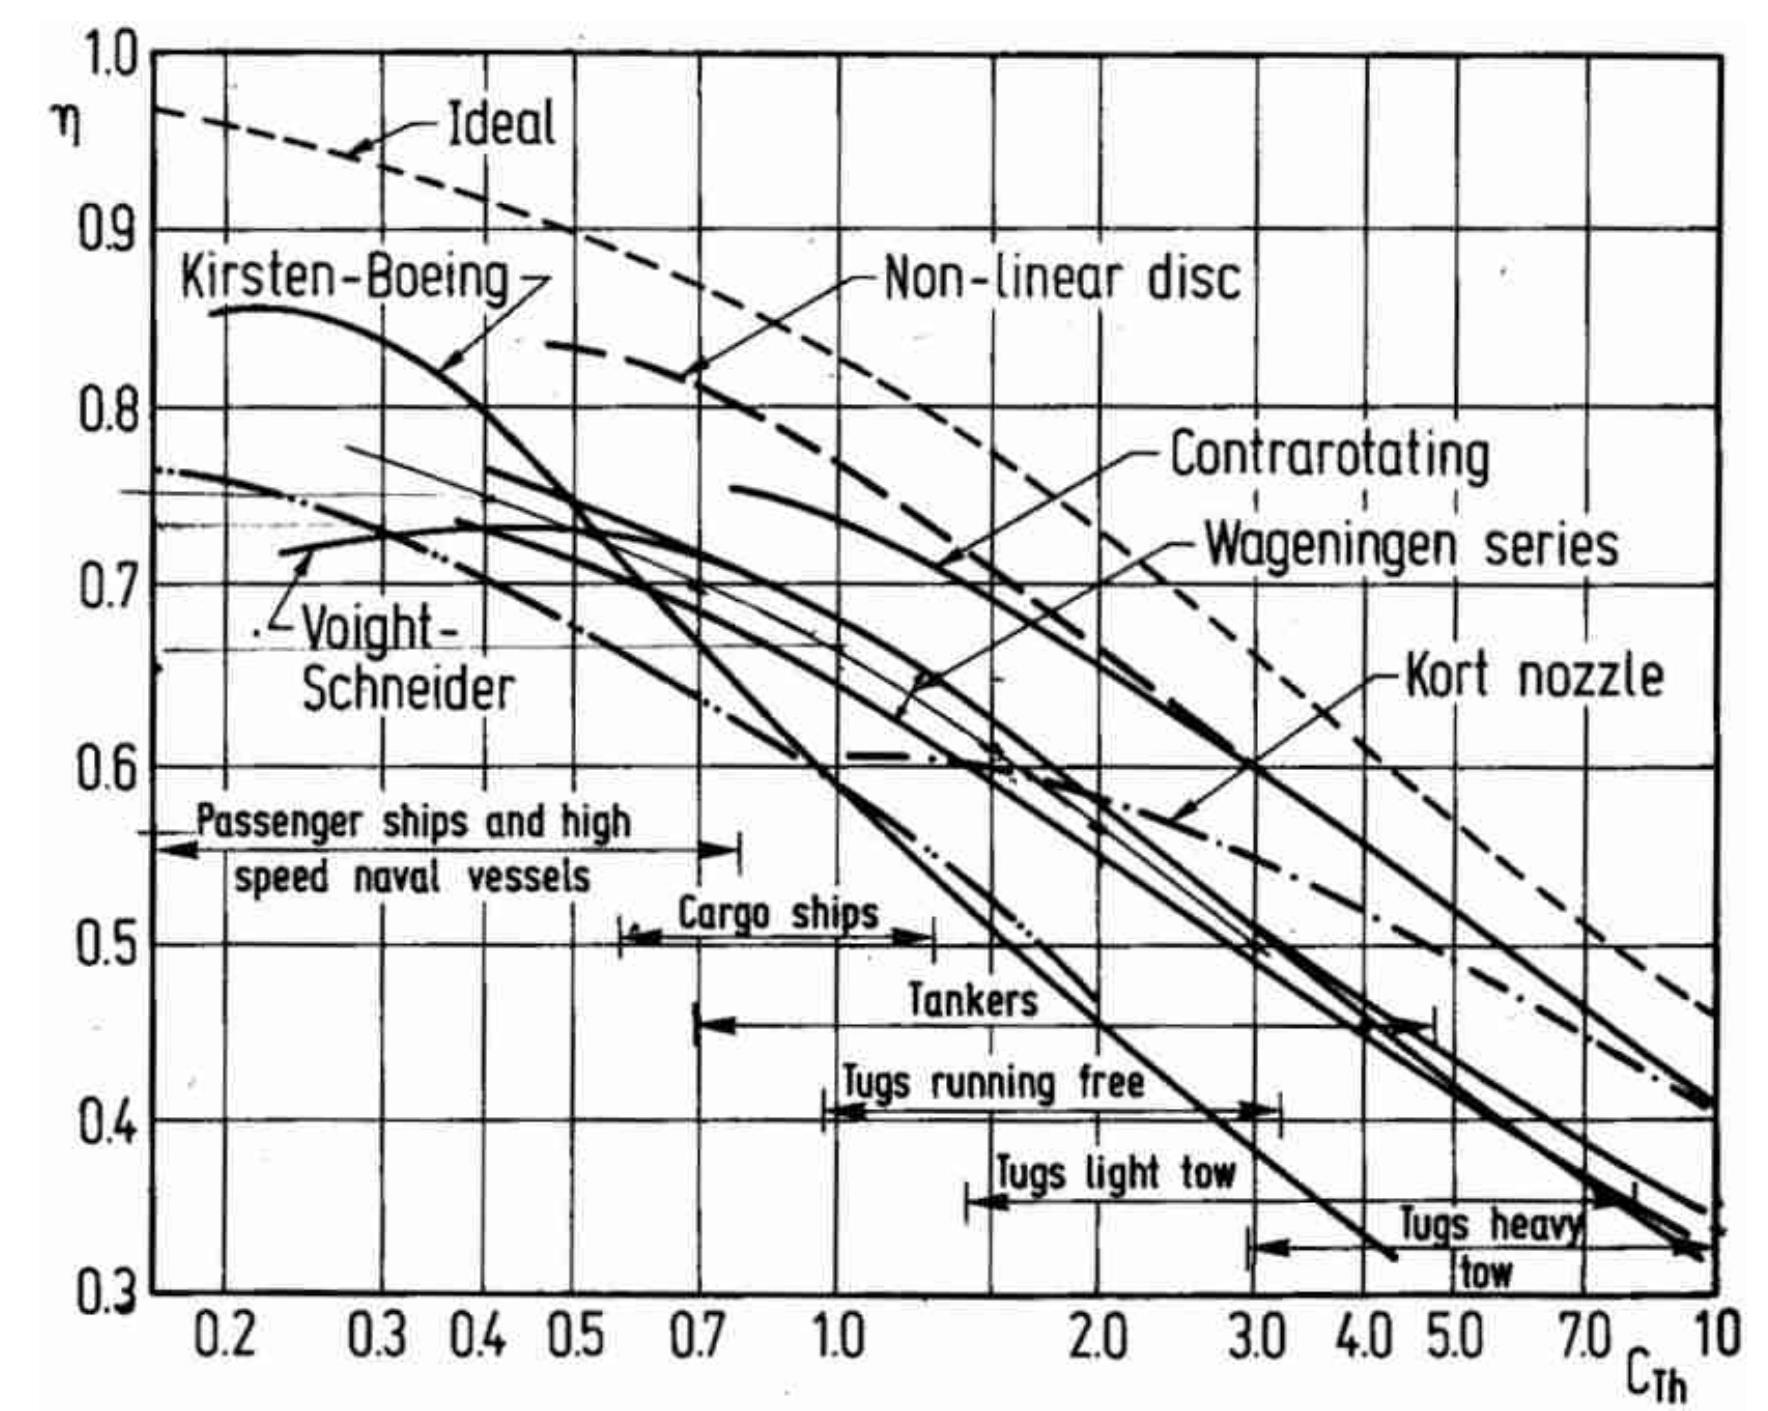
\includegraphics[width=.5\textwidth]{00_figures/Breslin94_openwater_eff.jpg}
  \caption{Efficiencies of various propulsion devices \citep{Breslin.1994}}
  \label{fig:breslin_open water efficiencies}
\end{figure}

The Hull efficiency $\eta_H$ can be calculated using the following equation:

\begin{equation}
    \label{eqn:hull_eff}
    \eta_H = \frac{1 - t}{1 - w_S}
\end{equation}

The term $t$ refers to the thrust deduction fraction, which represents the thrust force required to overcome the towing resistance of the ship $R_{TOTAL}$ and the additional resistance caused by the propeller's interaction with the hull. On the other hand, the term $w_S$ corresponds to the wake fraction, characterising the influence of the ship's hull on the water flow into the propeller \citep{Diesel.2011,Birk.2019}. The following equations are presented for twin-screw vessels.

\begin{equation}
    \label{eqn:wake_ws}
    w_S = 0.3095 C_B + 10 C_V C_B -0.23 \frac{D}{\sqrt{BT}}
\end{equation}

\begin{equation}
    \label{eqn:thrust_t}
    t = 0.325 C_B - 0.1885 \frac{D}{\sqrt{BT}}
\end{equation}

where $C_V$ is the viscous resistance coefficient, which combines all friction-related components of the resistance and the correlation resistance:

\begin{equation}
    \label{eqn:C_V}
    C_V = \frac{(1+k_1)R_F+R_{APP}+R_A}{\frac{1}{2}\rho v_S^2 (S+\sum_i S_{APP_i})}
\end{equation}

The relative rotative efficiency \begin{math} \eta_R \end{math} can be expressed by the following ratio, with $v_A$ defined as the arriving water velocity to propeller \citep{Diesel.2011}:

\begin{equation}
    \label{eqn: n_rot_MAN}
    \eta_R = \frac{\text{Power absorbed in open water at }v_A}{\text{Power absorbed in wake behind the ship at }v_A}
\end{equation}

According to \citet{Holtrop.1982}, $\eta_R$ for twin screw vessels can be estimated using the following formula, with $P/D$ defined as the propeller pitch-to-diameter ratio:

\begin{equation}
    \label{eqn: eta_rot_holtrop}
    \eta_R = 0.9737 + 0.111(C_P-0.0225\ell_{CB}) - 0.06325\frac{P}{D}
\end{equation}

The shaft efficiency \begin{math}\eta_S\end{math} is defined as the ratio between the power delivered to the propeller $P_D$ and the brake power of the main engine $P_B$, with values ranging from $\eta_S = 0.95 - 0.99$ depending on shaft design and gear configuration.


\subsubsection{Selection and validation of optimal model}\label{sec:select_and_val_model}

To ensure a meaningful assessment of the model's performance and its accuracy, the k-fold cross-validation technique will be employed. K-fold cross-validation involves partitioning the training set into k subsets, referred to as folds. The model will then undergo k training iterations, with each iteration using k-1 folds for training and the remaining fold for validation. During each iteration, the model's performance will be evaluated using various metrics, including the Coefficient of Determination ($R^2$), Explained Variance (EV), Mean Absolute Error (MAE), Root Mean Square Error (RMSE), Median Absolute Deviation (MAD), and Mean Absolute Percentage Error (MAPE). The results from each iteration will be averaged, providing an assessment of the model's accuracy, which can be further understood by considering the standard deviation. The utilization of k-fold cross-validation facilitates the evaluation of the model's robustness across different datasets.

\begin{figure}
  \centering
  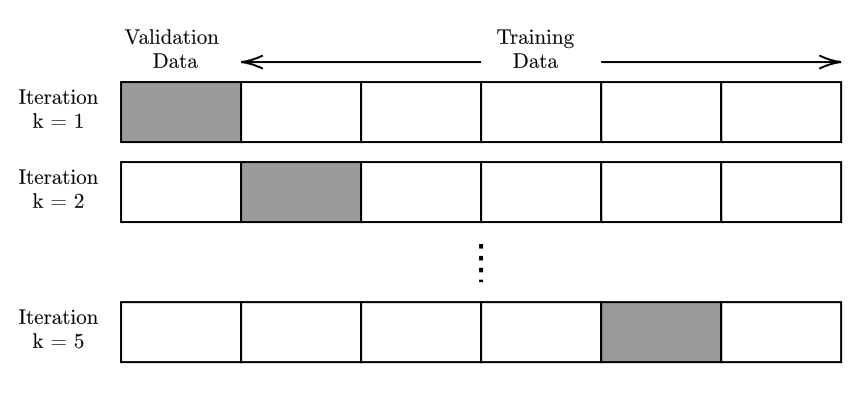
\includegraphics[width=.65\textwidth]{00_figures/kfold.png}
  \caption{Visual illustration of k-folding, Grey shaded box represents the validation data while white box represents the training data}
  \label{fig:kfold}
\end{figure}

\begin{equation}\label{eqn:rsquared}
  R^2(y,\hat{y}) = 1 - \frac{\sum_{i = 1}^{n} (y_{\text{i}} - \hat{y}_{\text{i}} )^2 }{\sum_{i = 1}^{n} (y_{\text{i}} - \overline{y}_{\text{i}})^2} \quad \textbf{where} \quad \overline{y} = \frac{1}{n}\sum_{1}^{n} y_\text{i}
\end{equation}

\begin{equation}\label{eqn:expVar}
  EV(y,\hat{y}) = 1 - \frac{\sigma^2_{(y-\hat{y})}}{\sigma^2_{y}}
\end{equation}

\begin{equation}\label{eqn:MAE}
  MAE(y,\hat{y}) = \frac{1}{n}\sum_{i=1}^{n} |y_{\text{i}} - \hat{y}_{\text{i}}| 
\end{equation}

\begin{equation}\label{eqn:RMSE}
  RMSE(y,\hat{y}) = \sqrt{\frac{1}{n}\sum_{i=1}^{n} (y_{\text{i}} - \hat{y}_{\text{i}})^2} 
\end{equation}

\begin{equation}\label{eqn:MAD}
  MAD(y,\hat{y}) =  \text{median} (|y_{\text{1}} - \hat{y}_{\text{1}}|,\dots,|y_{\text{i}} - \hat{y}_{\text{i}}|)
\end{equation}

\begin{equation}\label{eqn:MAPE}
  MAPE(y,\hat{y}) = \frac{1}{n}\sum_{i=1}^{n} \biggl|\frac{y_{\text{i}} - \hat{y}_{\text{i}}}{y_i}\biggr| \cdot 100\% 
\end{equation}

\section{Methodology Application}\label{sec:method_apply}

For further clarity regarding the methodology, the following steps are taken which are based on the proposed methodology. For generation of the BBM, the steps taken are: 

\begin{enumerate}
    \item Dataset is loaded.
    \item Identify and remove any anomalies.
    \item Remove static and unneeded features.
    \item Apply speed threshold of 5 knots.
    \item Highly correlated features are combined/removed based on physical and statistical reasoning.
    \item Impute missing values using {\tt KNNImputer}.
    \item Split the dataset into training and testing.
    \item Train the model using the whole dataset with the default hyperparameter.
    \item Evaluate model performance using k-fold cross-validation.
    \item Tune the model until the best model is obtained.
    \item For the case study, the best models will be used to predict the SOG using the test dataset.
\end{enumerate}

Subsequently, for FOC calculation, the following steps are taken:

\begin{enumerate}
    \item The test dataset is split into seasonal data. Summer-Fall season and Winter-Spring season corresponding to data for 6 months respectively.
    \item Impute missing values using {\tt KNNImputer}.
    \item SOG is converted to STW.
    \item Calculate calm water resistance $R_{CALM}$.
    \item Calculate added resistance due to wave $R_{AW}$.
    \item Calculate added resistance due to wind $R_{AA}$.
    \item Calculate total effective power $P_E$ using total resistance $R_{TOTAL}$.
    \item Calculate brake power $P_B$ from total efficiencies.
    \item Plot resulting regression line for Power-Speed curve from all models and actual case. 
    \item Calculate the FOC by considering the engine SFOC and operation time.
    \item Plot resulting regression line for FOC-Speed curve from all models and actual case.
    \item Evaluate the performance of the model generated from the regression lines.
\end{enumerate}

The dataset used in the case study will represent the journey of the ferry between K{\o}ge and R{\o}nne. After data preprocessing and cleaning. There are 3828 data points. The dataset is divided into training and test datasets with a ratio of 75:25 for training and testing, respectively. This results in 2871 data points for training and 957 data points for testing.

\section{Result and Discussion}\label{sec:research_discussion_j}

\subsection{Model Optimisation}\label{sec:hpo_journal}

From \texttt{GridSearchCV}, it cam be observed that the most optimal model shown in Figure \ref{tbl:hpo_optimal} can reduce the training time. This is most notably caused by limiting the depth of the tree, from \texttt{max\_depth = None} to \texttt{max\_depth = 100}. Table \ref{tbl:cv_rfr_j} and Figure \ref{fig:learn_curve_RFR_MAE} shows that the process of hyperparameter tuning for the Random Forest Regressor (RFR) model did not show any significant improvement in model performance. This outcome aligns with the findings of \citet{Kuhn.2013} and \citet{Hastie.2009}.

\begin{table}
  \tbl{Optimal hyperparameter with training time of each model}
    % \footnotesize
    % \centering
    % \resizebox {\textwidth}{!}
    {\begin{tabular}{ p{0.1\linewidth} p{0.2\linewidth}  p{0.3\linewidth} p{0.25\linewidth}}
    \hline
    Model & Training time [s] &  Optimal Hyperparameter & Search Range \\
    \hline
    RFR & 4.112 & None \\
    $\text{RFR}_{OPT}$ & 3.431  & {\tt min\_samples\_split = 2} & [2,10]\\
    &&{\tt min\_samples\_leaf = 1} & [1,10]\\
    &&{\tt max\_features = 10} & [6,12]\\
    &&{\tt max\_depth = 120} & [10,200] and [None]\\
    &&{\tt n\_estimators = 100} & [100,1000]\\
    \hline
    \end{tabular}}
  \label{tbl:hpo_optimal}
\end{table}

\begin{table}
\tbl{Cross Validation results of Random Forest (RF) Regressor}
    % \footnotesize
    % \centering
    % \resizebox {\textwidth}{!}
    {\begin{tabular}{l l c c}
    \hline
    Model   &       & RFR   	& $\text{RFR}_{OPT}$  \\
    \hline
    $R^2$   & [\%]  & 89.17   & 89.46               \\
    expVar  & [\%]  & 89.21   & 89.50               \\
    MAE     & [kn]  & 0.656   & 9.649               \\
    RMSE    & [kn]  & 1.015   & 1.008               \\
    MAD     & [kn]  & 0.446   & 0.445               \\  
    \hline
    \end{tabular}}
  \label{tbl:cv_rfr_j}
  \end{table}

\begin{figure}
    \centering
    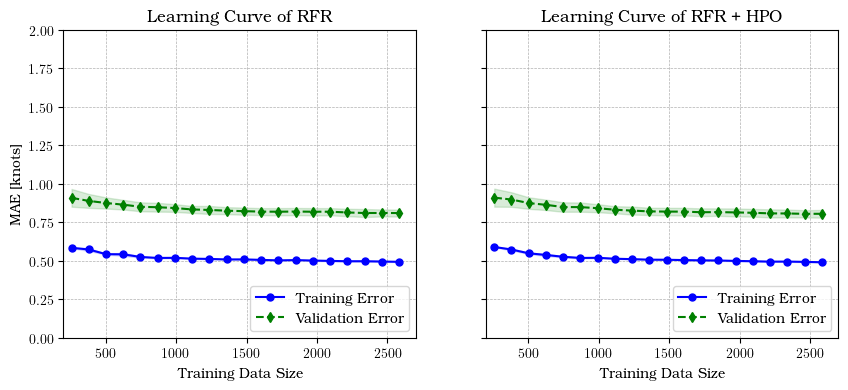
\includegraphics[width=.8\linewidth]{00_figures/learning_curve_rfr_mae.png}
    \caption{Learning curve of Random Forest (RF) Regressor}
    \label{fig:learn_curve_RFR_MAE}
\end{figure}

\subsection{Evaluation of Random Forest Regressor}\label{sec:testing_discission_j}

The optimised model will be assessed by testing its performance on a dataset comprising 957 data points from the entire year 2021, labelled as $DS_{year}$. To examine how different data points impact model performance, the dataset is split into two distinct seasons: $DS_{summer}$, covering May 2021 to October 2021, containing 454 data points; and $DS_{winter}$, including data from January 2021 to April 2021, and November 2021 to December 2021, totalling 503 data points. Missing values within the testing dataset will be handled using the {\tt KNNImputer} method.

\begin{table}
\tbl{Descriptive statistics of $DS_{year}$}
  % \footnotesize
  % \centering
  % \resizebox {\textwidth}{!}
  {\begin{tabular}{ p{0.21\linewidth} c c c c c c c c }
  \hline
  Features & Count & Mean & Std. & Min & 25\% & 50\% & 75\% & Max \\
  \hline
  \textbf{{\tt sog}} & 957.00 & 16.99 & 3.10 & 5.10 & 16.68 & 18.05 & 18.72 & 21.00\\
  \hline
  {\tt cog} & 957.00 & 196.73 & 86.72&	56.02 & 102.32& 185.22& 282.18& 319.85\\ 
  {\tt heading} & 957.00 & 188.30&	89.17&	63.49&	100.86&	124.24&	279.38&	308.04\\
  {\tt draught} & 957.00 & 5.23 & 0.19& 4.74& 5.11& 5.29& 5.38&5.66\\
  {\tt windspeed} & 957.00 & 6.45 & 3.04 & 0.40 & 4.11 & 6.13 &	8.21 & 15.85\\
  {\tt oceantemperature} & 957.00 & 282.28 & 6.48 & 267.25& 276.80& 281.91& 288.42& 295.70 \\
  {\tt waveperiod} & 957.00 & 3.69 & 0.88 & 1.67 & 3.06& 3.55& 4.22& 7.01\\
  {\tt surftemp} & 957.00 &283.20& 5.72& 273.15& 277.98& 282.65& 288.82 &294.93\\
  {\tt windwaveswellheight} &  957.00 & 0.77 & 0.54 & 0.08 &0.37 &0.63 &	0.95 &  3.24  \\
  {\tt curspeed} & 957.00 &0.09 & 0.07& 0.00 & 0.05& 0.07 & 0.13 & 0.50\\
  {\tt truewinddir} & 957.00 & 91.39 & 56.23 &	0.03 & 38.80 &	95.25 & 142.83 & 179.86\\
  {\tt truecurrentdir} & 957.00 & 90.75 & 57.76 & 0.26 & 31.52 & 90.44 & 144.65 & 179.95 \\
  {\tt truewavedir} & 957.00 & 86.79 & 55.76& 0.06& 35.81 & 82.32 & 138.93 & 179.81 \\
  \hline
  \end{tabular}}
% \caption{Descriptive statistics of $DS_{year}$}
\label{tbl:testyear_dataset_descriptive}
\end{table}

The results of SOG prediction of optimised RFR on optimised model are summarised in Table \ref{tbl:testing_dataset_sog_result}. Each model is tested against 3 different testing datasets, the yearly dataset $DS_{year}$, summer dataset, $DS_{summer}$ and winter dataset $DS_{winter}$. The performance of the random forest is compared against Multiple Linear Regressor (MLR) model.

\begin{table}
\tbl{Performance indices for SOG predictions}
  % \footnotesize
  % \small
  % \centering
  % \resizebox {\textwidth}{!}
  {\begin{tabular}{ l l c c c c c c }
  \hline
  Model & Dataset & $R^2$ & expVar & MAE & RMSE & MAD & MAPE \\
  & & [$\%$] & [$\%$] & [$kn$] & [$kn$] & [$kn$] & [$\%$]  \\ 
  \hline
  $\text{RFR}_{OPT}$ & $DS_{year}$  & 90.10 & 90.13 & 0.619 & 0.974 & 0.417 & 4.29 \\
  & $DS_{winter}$ & 93.41 & 93.53 & 0.548 & 0.832 & 0.372 & 3.94 \\
  & $DS_{summer}$ & 85.48 & 85.48 & 0.693 & 1.108 & 0.452 & 4.63 \\
  MLR & $DS_{year}$ & 69.57 & 69.62 & 1.147 & 1.709 & 0.917 & 7.75 \\
  & $DS_{winter}$ & 67.82 & 67.83 & 1.133 & 1.838 & 0.875 & 8.05 \\
  & $DS_{summer}$ & 71.24 & 71.63 & 1.159 & 1.559 & 0.952 & 7.38 \\
  \hline
  \end{tabular}}
% \caption{Performance indices for SOG predictions}
\label{tbl:testing_dataset_sog_result}
\end{table}

The results show that RFR is able to generally make good predictions across different datasets and show considerable robustness as indicated by the variance between the best and the worst result. With the $DS_{winter}$ dataset, RF regressor is able to showcase the best performance, achieving $R^2$ score of 93.41 \% and MAPE of 3.94\%. The result also showcase that the performance of the model is not only dependent on the quantity of the data, but it is also dependent on the quality of the data as well.

The results show that RFR consistently generates accurate predictions across various datasets, displaying notable robustness evident in the variance between the best and worst prediction results. In the case of the $DS_{winter}$ dataset, the RF regressor exhibits the best performance, attaining $R^2$ score of 93.41\% and a MAPE of 3.94\%. These findings also demonstrated that the model's effectiveness is influenced not solely by data quantity, but also by data quality.

To further understand the structure of the RF regressor, a feature importance plot is generated. Excluding ship heading and COG. The ship draught $T$ emerges as a significant factor influencing the prediction of SOG. This aligns with the theory of frictional resistance $R_F$ encountered by the ship, which is a function of the wetted surface area of bare hull $S$. Deeper draught $T$ will result in more submerged area of the hull and this will consequently increase the frictional force $R_F$ of the ship. Given a constant supply of power to the ship propulsion system, the speed of the ship will decrease.

\begin{figure}
  \centering
  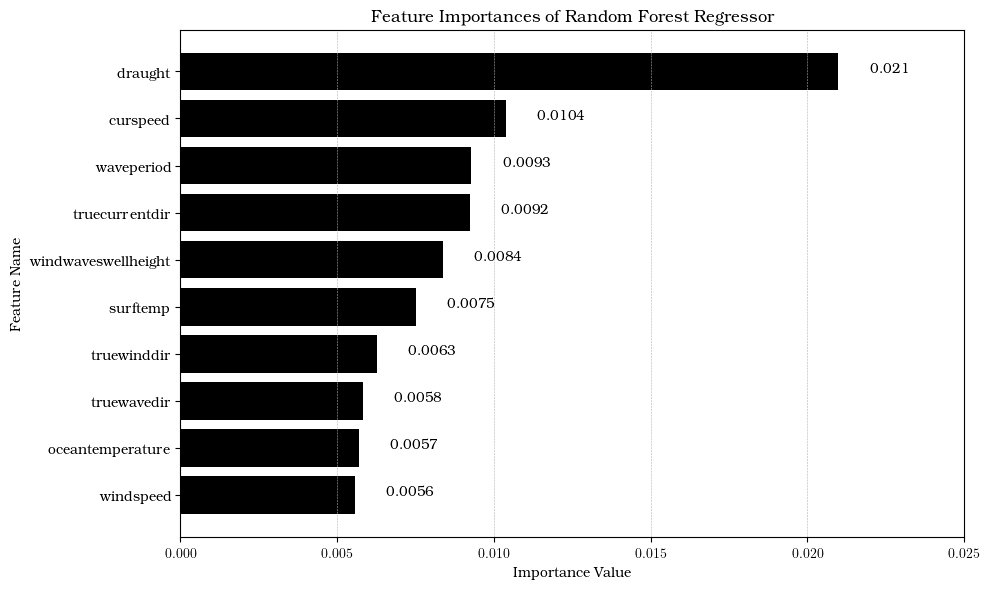
\includegraphics[width=.8\linewidth]{00_figures/rfr_ftr_importance_nodir.png}
  \caption{Learning curve of Random Forest (RF) Regressor}
  \label{fig:learn_curve_RFR_MAE}
\end{figure}

Regarding weather conditions, RFR models highlight current-based variables like current speed and true current direction as the most influential factors affecting SOG prediction. This observation aligns with the suggested approach for current correction, which emphasizes the importance of considering both current magnitude and direction when converting SOG to STW. Following these, the subsequent significant attributes according to the rankings of the RFR models are wave-related parameters: significant wave height ($H_{1/3}$), true wave direction, and wave period ({\tt waveperiod}). This agreement corresponds to the additional resistance generated by waves ($R_{AW}$) in the computation of the total resistance ($R_{TOTAL}$) experienced by the ship. Wind-related factors, including wind speed and true wind direction, contribute to the added resistance caused by wind force ($R_{AA}$). However, these aspects have the least impact on SOG prediction.

\begin{figure}
  \label{fig:dtr_tree_trained}
  \centering
  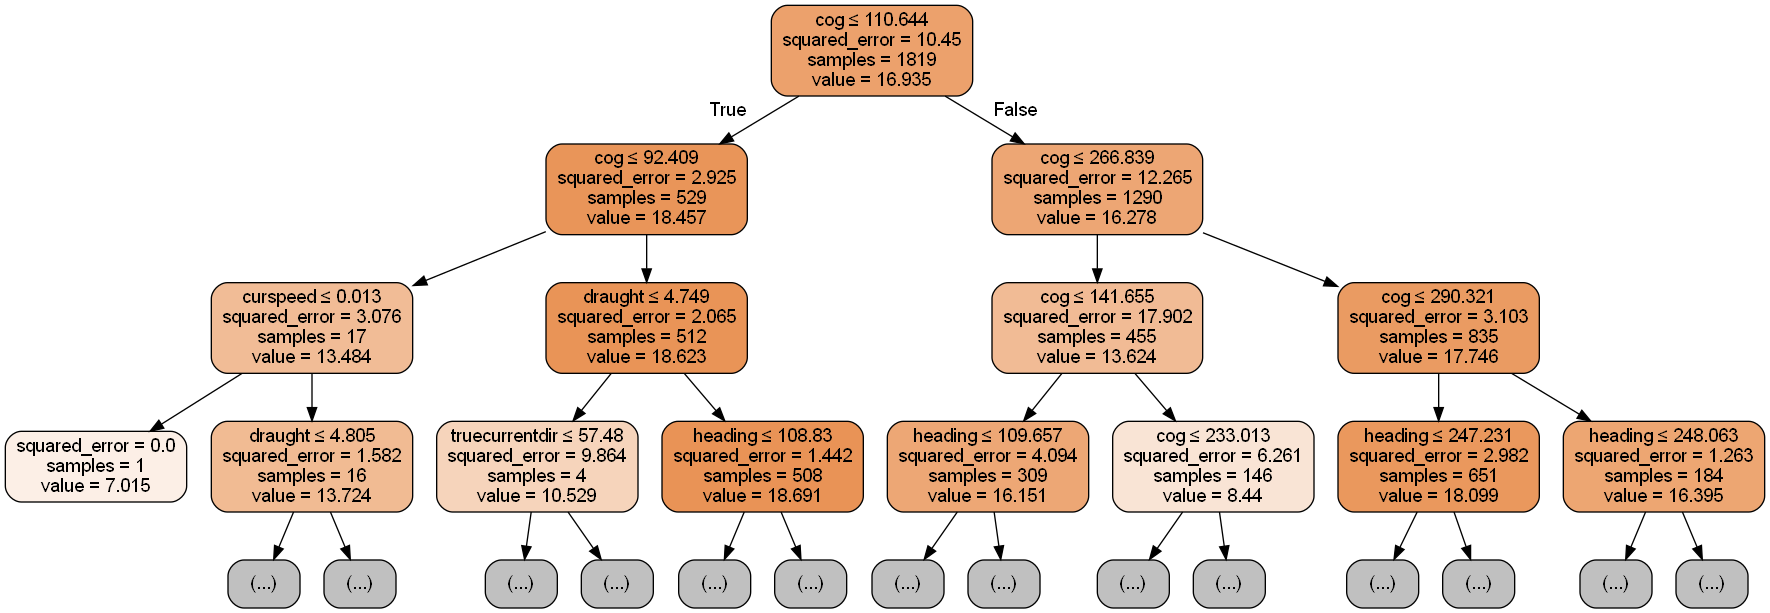
\includegraphics[width=.9\textwidth]{00_figures/rfr_mod_it1.png}
  \caption{Partial structure of RF Regressor}
\end{figure}

\subsection{Evaluation of the power estimation method}\label{sec:power_estimate_eval_j}

Table \ref{tbl:FOC_scores_errors} presents the results for FOC prediction of RF Regressor. Notably, there is a decline in the $R^2$ score and MAPE for the RFR. This decrease in performance could be attributed to the inherent nonlinearity of the WBM, which tends to amplify FOC prediction errors at higher ship speeds. This phenomenon is exemplified by the case study conducted by \citet{Birk.2019}. In the case study, a discrepancy of $1$ knot in ship speed resulted in a power difference of around $1200$ kW at lower speeds. However, at higher speeds, the power difference escalated to about $2300$ kW. Nevertheless, the FOC prediction is still reasonable, achieving $R^2$ score of 86.57\% and MAPE of 12.06\%.

\begin{table}
\tbl{Performance indices for FOC prediction}  
  % \footnotesize
  % % \small
  % \centering
  % \resizebox {\textwidth}{!}
  {\begin{tabular}{ l l c c c c c c }
  \hline
  Model & Dataset & $R^2$ & expVar & MAE & RMSE & MAD & MAPE \\
  & & [$\%$] & [$\%$] & [$T/h$] & [$T/h$] & [$T/h$] & [$\%$]  \\ 
  \hline
  $\text{RFR}_{OPT}$ & $DS_{year}$  & 81.81 & 81.87 & 0.117 & 0.171 & 0.079 & 13.64 \\
  & $DS_{winter}$ & 86.57 & 86.58 & 0.099 & 0.141 & 0.068 & 12.06 \\
  & $DS_{summer}$ & 76.82 & 77.20 & 0.137 & 0.198 & 0.088 & 15.31 \\
  MLR & $DS_{year}$ & 29.16 & 31.81 & 0.223 & 0.337 & 0.171 & 29.39 \\
  & $DS_{winter}$ & 10.39 & 11.37 & 0.212 & 0.363 &0.161& 33.19 \\
  & $DS_{summer}$ & 44.33 & 49.66 & 0.235 & 0.307 & 0.191 & 25.24 \\
  \hline
  \end{tabular}}
% \caption{Performance indices for FOC prediction}
\label{tbl:FOC_scores_errors}
\end{table}

The resulting bunker-to-speed curve plots are displayed in Figure \ref{fig:foc_curve_rfr_dsyear}. These resulting functions are in alignment with the findings reported by \citet{Psaraftis.2013}. According to the cubic law, the fuel consumption rate can be represented by a proportional factor multiplied by the sailing speed raised to the power of $\alpha = 3$ \citep{Du.2019}. However, \citet{Psaraftis.2013} noted that the cubic law might not be valid for low speeds, and the factor $\alpha$ could be 4, 5, or even higher for specific ship types or when operating at high speeds.

\begin{figure}
  \label{fig:foc_curve_rfr_dsyear}
  \centering
  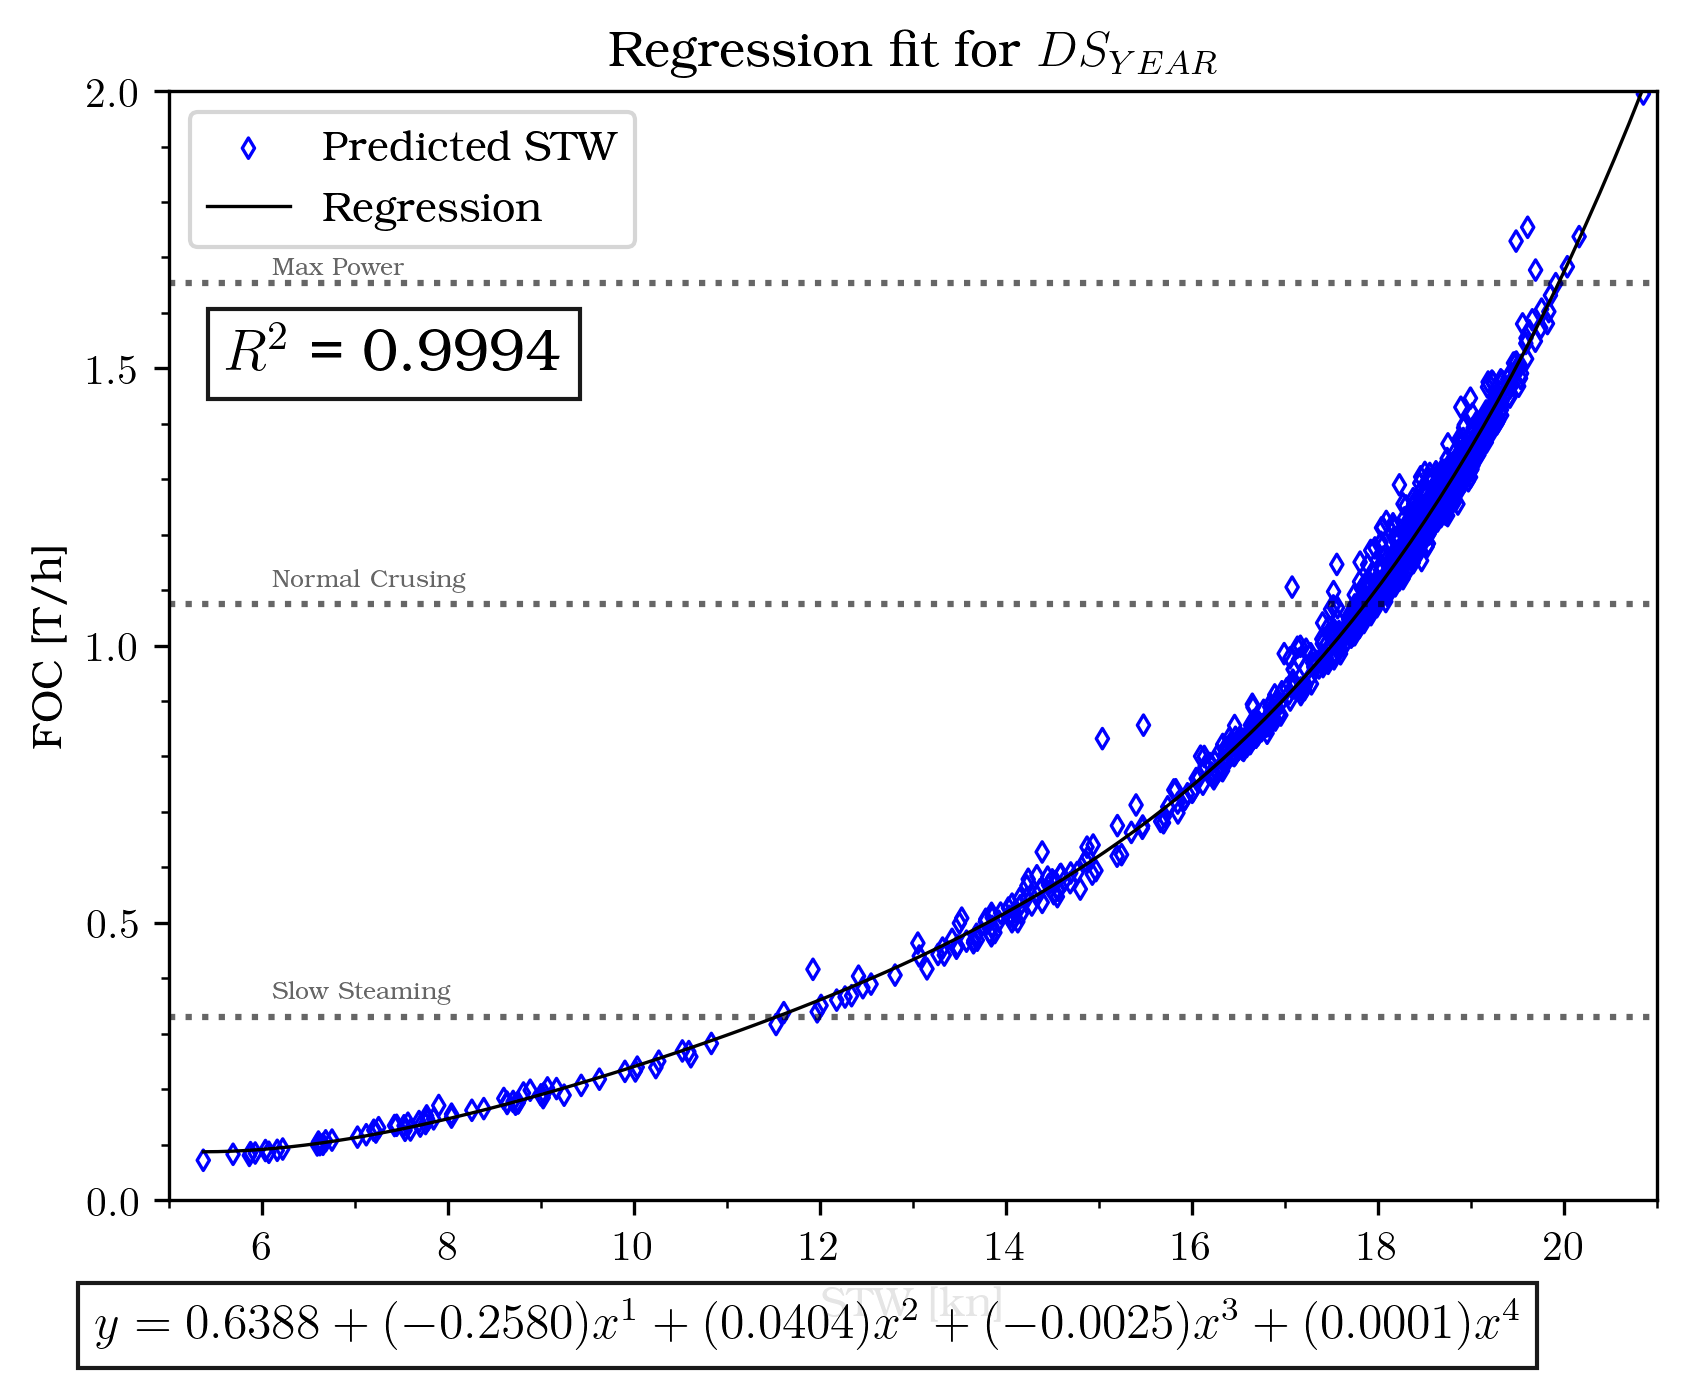
\includegraphics[width=.8\textwidth]{00_figures/rfr_year_foccurve.png}
  \caption{Generated FOC to speed curve for dataset $DS_{year}$}
\end{figure}

The FOC to speed curve also reveal situations where the model predicts ship speeds surpassing the maximum engine rating, a physically impossible scenario. This concern arises from the conversion of SOG to STW. By analysing publicly available data from the study conducted by \citet{JoanPeturPetersen.2011}\footnote{http://cogsys.imm.dtu.dk/propulsionmodelling/}, a noticeable divergence between SOG and STW becomes apparent, typically differing by a factor of around 0.85. Even after incorporating current correction in this case study, the speed difference remains slight. This implies that the conversion of SOG to STW should also account for the impact of speed reduction due to wind and waves. Direct speed loss formulas for wind and wave effects are presented by \citet{Aertssen.1975} and \citet{kwon.2008}. However, these formulas have limited applicability ranges and are not optimized for different vessel types.

\subsection{Key Findings}\label{sec:key_finding}

\subsubsection{Performance of BBM}

\begin{itemize}
  
\item RFR is able to perform reasonable SOG prediction, achieving $R^2$ score of 93.41\% and a MAPE of 3.94\%. A simple MLR model may be insufficient for implementation, as a substantial performance gap is found between MLR and other tree-based models, with $R^2$ score of $72\%$ and MAE of 1.16 knots.

\item The quality and quantity of data are closely interrelated factors that significantly impact model performance. There are noticeable differences in the performance between the $DS_{winter}$ and $DS_{summer}$ datasets, with an increase of approximately $6\%$ in the $R^2$ score and a reduction of about 0.1 knots in MAE is achievable with an increase in about 50 data points.

\item However, the quantity of data alone is insufficient to ensure an increase in model performance. This observation is evident from the $DS_{year}$ datasets, which contain approximately twice as much data as the other datasets, yet the model's performance is not superior to that of the $DS_{winter}$ dataset. This suggests that the quality of the $DS_{summer}$ dataset may compromise the model's performance when using the $DS_{year}$ dataset.

\item The impact of optimization on RFR and ETR models is minimal. Analysing feature importances and model structure visualisation, the RFR model recognizes draught as the most influential factor affecting SOG prediction. While the ETR and DTR models also identify this factor, but with a lesser degree of recognition.

\end{itemize}

\subsubsection{Performance of power estimation method}

\begin{itemize}

\item Due to the sequential approach of GBM, the predictive performance of BBM is carried over to WBM during FOC prediction. RFR is able to achieve a $R^2$ score of 86.57\% and MAPE of 12.06\%. 

\item The nonlinear relation between speed and bunker means that significant deviation of SOG leads to an amplified magnitude of errors for FOC. This is evident in the case of MLR, the model already made relatively larger errors than other tree-based models during SOG prediction. With that, it is important to ensure that the SOG prediction of BBM is to be optimised as much as possible to ensure accurate FOC prediction. 

\item The power estimation method by Holtrop-Mennen method resulted in a 4\textsuperscript{th} order bunker-to-speed function.
 
\end{itemize}

\section{Conclusion}

This study proposed a comprehensive approach that combines data-driven techniques with empirical models to estimate FOC for a sailing vessel. The optimised machine learning model effectively forecasts FOC for vessels navigating at varying speeds, draughts, and weather conditions. The outcomes substantiate the viability of integrating AIS data and weather data for SOG prediction, which will then be used for FOC estimation. Technical details about the ship can be derived from AIS data. Along with suitable approximations from suitable and relevant literature, FOC can be forecasted using the empirical formulas proposed by Holtrop-Mennen. The results of predicted FOC can be used to generate bunker-to-fuel functions to estimate FOC for varying STW. The main findings are summarised in the following points.\\

\begin{itemize}
  \item Machine learning-based FOC models rely on feature engineering like feature selection and importance identification. High correlation filter analysis is a common approach, removing highly correlated features. Removing a feature should primarily be based on the understanding of physical and vessel-related knowledge.
  \item Hourly AIS data resolution offers an advantage over noon data, especially for predicting within shorter periods. The hourly model in this study effectively forecasts FOC within seasonal or yearly intervals.
  \item Holtrop-Mennen method is a viable method for estimating energy for operation. The introduction of this empirical model ensures adherence to physical principles of the vessel. Missing input values can be approximated using formulas or similar cases. However, approximations introduce errors; interpolation using measurements from towing tank resistance test data is preferred.
  \item The Random Forest Regressor effectively predicts SOG in the Black Box Model. This approach requires minimal data pre-processing and model configuration. Tree-based models' feature importance aids in implicit feature selection. 
  \item Integrating the White Box Model diminishes the domain knowledge-free advantage of the Black Box Model, and the sequential approach may propagate prediction errors during energy estimation.
\end{itemize}

\section*{Replication and data sharing}

Readers can find the computer code and dataset used in this study in the provided URL: https://github.com/hiwafi/thesis-ais.git. 

\section*{Disclosure statement}

The authors declare that they have no known competing financial interests or personal relationships that could have appeared to influence the work reported in this paper.


\bibliographystyle{tfcad}
\bibliography{interactcadsample}

% \section{Using the \texttt{interact} class file}

% For convenience, simply copy the \texttt{interact.cls} file into the same directory as your manuscript files (you do not need to install it in your \TeX\ distribution). In order to use the \texttt{interact} document class, replace the command \verb"\documentclass{article}" at the beginning of your document with the command \verb"\documentclass{interact}".

% The following document-class options should \emph{not} be used with the \texttt{interact} class file:
% \begin{itemize}
%   \item \texttt{10pt}, \texttt{11pt}, \texttt{12pt} -- unavailable;
%   \item \texttt{oneside}, \texttt{twoside} -- not necessary, \texttt{oneside} is the default;
%   \item \texttt{leqno}, \texttt{titlepage} -- should not be used;
%   \item \texttt{twocolumn} -- should not be used (see Subsection~\ref{class});
%   \item \texttt{onecolumn} -- not necessary as it is the default style.
% \end{itemize}
% To prepare a manuscript for a journal that is printed in A4 (two column) format, use the \verb"largeformat" document-class option provided by \texttt{interact.cls}; otherwise the class file produces pages sized for B5 (single column) format by default. The \texttt{geometry} package should not be used to make any further adjustments to the page dimensions.

% %If your manuscript has supplementary content you can prepare this using the \verb"suppldata" document-class option, which will suppress the `article history' date. This option must \emph{not} be used on any primary content.


% \section{Additional features of the \texttt{interact} class file}

% \subsection{Title, authors' names and affiliations, abstracts and article types}

% The title should be generated at the beginning of your article using the \verb"\maketitle" command.
% In the final version the author name(s) and affiliation(s) must be followed immediately by \verb"\maketitle" as shown below in order for them to be displayed in your PDF document.
% To prepare an anonymous version for double-blind peer review, you can put the \verb"\maketitle" between the \verb"\title" and the \verb"\author" in order to hide the author name(s) and affiliation(s) temporarily.
% Next you should include the abstract if your article has one, enclosed within an \texttt{abstract} environment.
% The \verb"\articletype" command is also provided as an \emph{optional} element which should only be included if your article actually needs it.
% For example, the titles for this document begin as follows:
% \begin{verbatim}
% \articletype{ARTICLE TEMPLATE}

% \title{Taylor \& Francis \LaTeX\ template for authors (\textsf{Interact}
% layout + Chicago author-date reference style)}

% \author{
% \name{A.~N. Author\textsuperscript{a}\thanks{CONTACT A.~N. Author.
% Email: latex.helpdesk@tandf.co.uk} and John Smith\textsuperscript{b}}
% \affil{\textsuperscript{a}Taylor \& Francis, 4 Park Square, Milton
% Park, Abingdon, UK; \textsuperscript{b}Institut f\"{u}r Informatik,
% Albert-Ludwigs-Universit\"{a}t, Freiburg, Germany} }

% \maketitle

% \begin{abstract}
% This template is for authors who are preparing a manuscript for a
% Taylor \& Francis journal using the \LaTeX\ document preparation system
% and the \texttt{interact} class file, which is available via selected
% journals' home pages on the Taylor \& Francis website.
% \end{abstract}
% \end{verbatim}

% An additional abstract in another language (preceded by a translation of the article title) may be included within the \verb"abstract" environment if required.

% A graphical abstract may also be included if required. Within the \verb"abstract" environment you can include the code
% \begin{verbatim}
% \\\resizebox{25pc}{!}{\includegraphics{abstract.eps}}
% \end{verbatim}
% where the graphical abstract is to appear, where \verb"abstract.eps" is the name of the file containing the graphic (note that \verb"25pc" is the recommended maximum width, expressed in pica, for the graphical abstract in your manuscript).


% \subsection{Abbreviations}

% A list of abbreviations may be included if required, enclosed within an \texttt{abbreviations} environment, i.e.\ \verb"\begin{abbreviations}"\ldots\verb"\end{abbreviations}", immediately following the \verb"abstract" environment.


% \subsection{Keywords}

% A list of keywords may be included if required, enclosed within a \texttt{keywords} environment, i.e.\ \verb"\begin{keywords}"\ldots\verb"\end{keywords}". Additional keywords in other languages (preceded by a translation of the word `keywords') may also be included within the \verb"keywords" environment if required.


% \subsection{Subject classification codes}

% AMS, JEL or PACS classification codes may be included if required. The \texttt{interact} class file provides an \texttt{amscode} environment, i.e.\ \verb"\begin{amscode}"\ldots\verb"\end{amscode}", a \texttt{jelcode} environment, i.e.\ \verb"\begin{jelcode}"\ldots\verb"\end{jelcode}", and a \texttt{pacscode} environment, i.e.\ \verb"\begin{pacscode}"\ldots\verb"\end{pacscode}" to assist with this.


% \subsection{Additional footnotes to the title or authors' names}

% The \verb"\thanks" command may be used to create additional footnotes to the title or authors' names if required. Footnote symbols for this purpose should be used in the order
% $^\ast$~(coded as \verb"$^\ast$"), $\dagger$~(\verb"$\dagger$"), $\ddagger$~(\verb"$\ddagger$"), $\S$~(\verb"$\S$"), $\P$~(\verb"$\P$"), $\|$~(\verb"$\|$"),
% $\dagger\dagger$~(\verb"$\dagger\dagger$"), $\ddagger\ddagger$~(\verb"$\ddagger\ddagger$"), $\S\S$~(\verb"$\S\S$"), $\P\P$~(\verb"$\P\P$").

% Note that any \verb"footnote"s to the main text will automatically be assigned the superscript symbols 1, 2, 3, etc. by the class file.\footnote{If preferred, the \texttt{endnotes} package may be used to set the notes at the end of your text, before the bibliography. The symbols will be changed to match the style of the journal if necessary by the typesetter.}


% \section{Some guidelines for using the standard features of \LaTeX}

% \subsection{Sections}

% The \textsf{Interact} layout style allows for five levels of section heading, all of which are provided in the \texttt{interact} class file using the standard \LaTeX\ commands \verb"\section", \verb"\subsection", \verb"\subsubsection", \verb"\paragraph" and \verb"\subparagraph". Numbering will be automatically generated for all these headings by default.


% \subsection{Lists}

% Numbered lists are produced using the \texttt{enumerate} environment, which will number each list item with arabic numerals by default. For example,
% \begin{enumerate}
%   \item first item
%   \item second item
%   \item third item
% \end{enumerate}
% was produced by
% \begin{verbatim}
% \begin{enumerate}
%   \item first item
%   \item second item
%   \item third item
% \end{enumerate}
% \end{verbatim}
% Alternative numbering styles can be achieved by inserting an optional argument in square brackets to each \verb"item", e.g.\ \verb"\item[(i)] first item"\, to create a list numbered with roman numerals at level one.

% Bulleted lists are produced using the \texttt{itemize} environment. For example,
% \begin{itemize}
%   \item First bulleted item
%   \item Second bulleted item
%   \item Third bulleted item
% \end{itemize}
% was produced by
% \begin{verbatim}
% \begin{itemize}
%   \item First bulleted item
%   \item Second bulleted item
%   \item Third bulleted item
% \end{itemize}
% \end{verbatim}


% \subsection{Figures}

% The \texttt{interact} class file will deal with positioning your figures in the same way as standard \LaTeX. It should not normally be necessary to use the optional \texttt{[htb]} location specifiers of the \texttt{figure} environment in your manuscript; you may, however, find the \verb"[p]" placement option or the \verb"endfloat" package useful if a journal insists on the need to separate figures from the text.

% Figure captions appear below the figures themselves, therefore the \verb"\caption" command should appear after the body of the figure. For example, Figure~\ref{sample-figure} with caption and sub-captions is produced using the following commands:
% \begin{verbatim}
% \begin{figure}
% \centering
% \subfigure[An example of an individual figure sub-caption.]{%
% \resizebox*{5cm}{!}{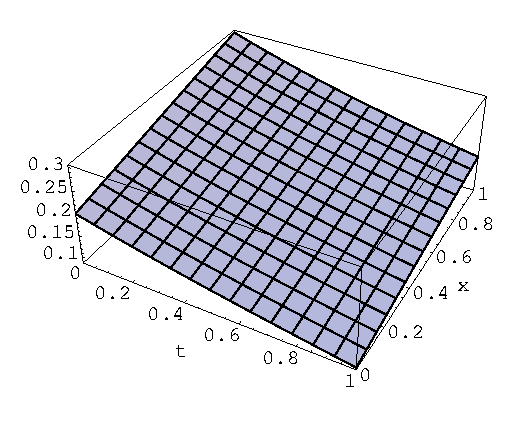
\includegraphics{graph1.eps}}}\hspace{5pt}
% \subfigure[A slightly shorter sub-caption.]{%
% \resizebox*{5cm}{!}{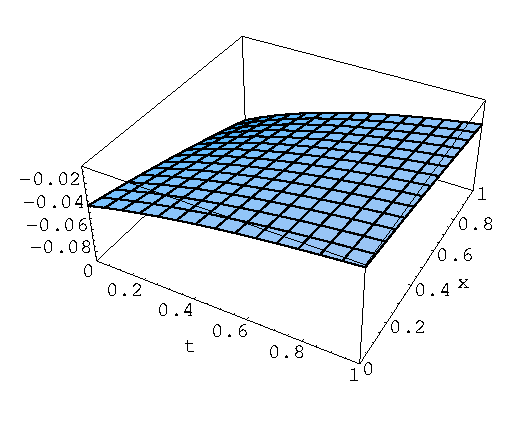
\includegraphics{graph2.eps}}}
% \caption{Example of a two-part figure with individual sub-captions
%  showing that captions are flush left and justified if greater
%  than one line of text.} \label{sample-figure}
% \end{figure}
% \end{verbatim}
% \begin{figure}
% \centering
% \subfigure[An example of an individual figure sub-caption.]{%
% \resizebox*{5cm}{!}{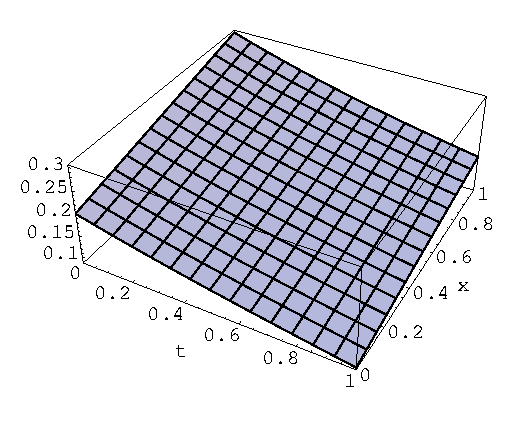
\includegraphics{graph1.eps}}}\hspace{5pt}
% \subfigure[A slightly shorter sub-caption.]{%
% \resizebox*{5cm}{!}{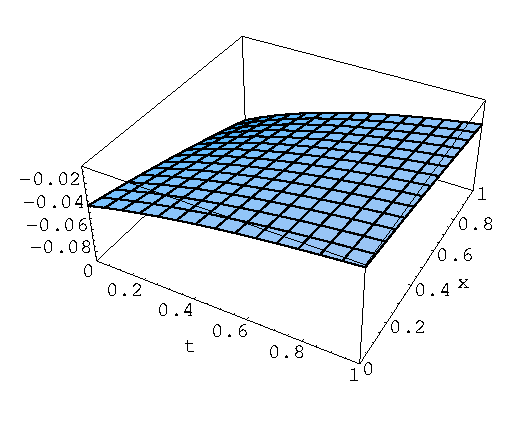
\includegraphics{graph2.eps}}}
% \caption{Example of a two-part figure with individual sub-captions
%  showing that captions are flush left and justified if greater
%  than one line of text.} \label{sample-figure}
% \end{figure}

% To ensure that figures are correctly numbered automatically, the \verb"\label" command should be included just after the \verb"\caption" command, or in its argument.

% The \verb"\subfigure" command requires \verb"subfigure.sty", which is called in the preamble of the \texttt{interacttfssample.tex} file (to allow your choice of an alternative package if preferred) and included in the \textsf{Interact} \LaTeX\ bundle for convenience. Please supply any additional figure macros used with your article in the preamble of your .tex file.

% The source files of any figures will be required when the final, revised version of a manuscript is submitted. Authors should ensure that these are suitable (in terms of lettering size, etc.) for the reductions they envisage.

% The \texttt{epstopdf} package can be used to incorporate encapsulated PostScript (.eps) illustrations when using PDF\LaTeX, etc. Please provide the original .eps source files rather than the generated PDF images of those illustrations for production purposes.


% \subsection{Tables}

% The \texttt{interact} class file will deal with positioning your tables in the same way as standard \LaTeX. It should not normally be necessary to use the optional \texttt{[htb]} location specifiers of the \texttt{table} environment in your manuscript; you may, however, find the \verb"[p]" placement option or the \verb"endfloat" package useful if a journal insists on the need to separate tables from the text.

% The \texttt{tabular} environment can be used as shown to create tables with single horizontal rules at the head, foot and elsewhere as appropriate. The captions appear above the tables in the \textsf{Interact} style, therefore the \verb"\tbl" command should be used before the body of the table. For example, Table~\ref{sample-table} is produced using the following commands:
% \begin{table}
% \tbl{Example of a table showing that its caption is as wide as
%  the table itself and justified.}
% {\begin{tabular}{lcccccc} \toprule
%  & \multicolumn{2}{l}{Type} \\ \cmidrule{2-7}
%  Class & One & Two & Three & Four & Five & Six \\ \midrule
%  Alpha\textsuperscript{a} & A1 & A2 & A3 & A4 & A5 & A6 \\
%  Beta & B2 & B2 & B3 & B4 & B5 & B6 \\
%  Gamma & C2 & C2 & C3 & C4 & C5 & C6 \\ \bottomrule
% \end{tabular}}
% \tabnote{\textsuperscript{a}This footnote shows how to include
%  footnotes to a table if required.}
% \label{sample-table}
% \end{table}
% \begin{verbatim}
% \begin{table}
% \tbl{Example of a table showing that its caption is as wide as
%  the table itself and justified.}
% {\begin{tabular}{lcccccc} \toprule
%  & \multicolumn{2}{l}{Type} \\ \cmidrule{2-7}
%  Class & One & Two & Three & Four & Five & Six \\ \midrule
%  Alpha\textsuperscript{a} & A1 & A2 & A3 & A4 & A5 & A6 \\
%  Beta & B2 & B2 & B3 & B4 & B5 & B6 \\
%  Gamma & C2 & C2 & C3 & C4 & C5 & C6 \\ \bottomrule
% \end{tabular}}
% \tabnote{\textsuperscript{a}This footnote shows how to include
%  footnotes to a table if required.}
% \label{sample-table}
% \end{table}
% \end{verbatim}

% To ensure that tables are correctly numbered automatically, the \verb"\label" command should be included just before \verb"\end{table}".

% The \verb"\toprule", \verb"\midrule", \verb"\bottomrule" and \verb"\cmidrule" commands are those used by \verb"booktabs.sty", which is called by the \texttt{interact} class file and included in the \textsf{Interact} \LaTeX\ bundle for convenience. Tables produced using the standard commands of the \texttt{tabular} environment are also compatible with the \texttt{interact} class file.


% \subsection{Landscape pages}

% If a figure or table is too wide to fit the page it will need to be rotated, along with its caption, through 90$^{\circ}$ anticlockwise. Landscape figures and tables can be produced using the \verb"rotating" package, which is called by the \texttt{interact} class file. The following commands (for example) can be used to produce such pages.
% \begin{verbatim}
% \setcounter{figure}{1}
% \begin{sidewaysfigure}
% \centerline{\epsfbox{figname.eps}}
% \caption{Example landscape figure caption.}
% \label{landfig}
% \end{sidewaysfigure}
% \end{verbatim}
% \begin{verbatim}
% \setcounter{table}{1}
% \begin{sidewaystable}
%  \tbl{Example landscape table caption.}
%   {\begin{tabular}{@{}llllcll}
%     .
%     .
%     .
%   \end{tabular}}\label{landtab}
% \end{sidewaystable}
% \end{verbatim}
% Before any such float environment, use the \verb"\setcounter" command as above to fix the numbering of the caption (the value of the counter being the number given to the preceding figure or table). Subsequent captions will then be automatically renumbered accordingly. The \verb"\epsfbox" command requires \verb"epsfig.sty", which is called by the \texttt{interact} class file and is also included in the \textsf{Interact} \LaTeX\ bundle for convenience.

% Please note that if the \verb"endfloat" package is used, one or both of the commands
% \begin{verbatim}
% \DeclareDelayedFloatFlavor{sidewaysfigure}{figure}
% \DeclareDelayedFloatFlavor{sidewaystable}{table}
% \end{verbatim}
% will need to be included in the preamble of your .tex file, after the \verb"endfloat" package is loaded, in order to process any landscape figures and/or tables correctly.


% \subsection{Theorem-like structures}

% A predefined \verb"proof" environment is provided by the \texttt{amsthm} package (which is called by the \texttt{interact} class file), as follows:
% \begin{proof}
% More recent algorithms for solving the semidefinite programming relaxation are particularly efficient, because they explore the structure of the MAX-CUT problem.
% \end{proof}
% \noindent This was produced by simply typing:
% \begin{verbatim}
% \begin{proof}
% More recent algorithms for solving the semidefinite programming
% relaxation are particularly efficient, because they explore the
% structure of the MAX-CUT problem.
% \end{proof}
% \end{verbatim}
% Other theorem-like environments (theorem, definition, remark, etc.) need to be defined as required, e.g.\ using \verb"\newtheorem{theorem}{Theorem}" in the preamble of your .tex file (see the preamble of \verb"interactcadsample.tex" for more examples). You can define the numbering scheme for these structures however suits your article best. Please note that the format of the text in these environments may be changed if necessary to match the style of individual journals by the typesetter during preparation of the proofs.


% \subsection{Mathematics}

% \subsubsection{Displayed mathematics}

% The \texttt{interact} class file will set displayed mathematical formulas centred on the page without equation numbers if you use the \texttt{displaymath} environment or the equivalent \verb"\[...\]" construction. For example, the equation
% \[
%  \hat{\theta}_{w_i} = \hat{\theta}(s(t,\mathcal{U}_{w_i}))
% \]
% was typeset using the commands
% \begin{verbatim}
% \[
%  \hat{\theta}_{w_i} = \hat{\theta}(s(t,\mathcal{U}_{w_i}))
% \]
% \end{verbatim}

% For those of your equations that you wish to be automatically numbered sequentially throughout the text for future reference, use the \texttt{equation} environment, e.g.
% \begin{equation}
%  \hat{\theta}_{w_i} = \hat{\theta}(s(t,\mathcal{U}_{w_i}))
% \end{equation}
% was typeset using the commands
% \begin{verbatim}
% \begin{equation}
%  \hat{\theta}_{w_i} = \hat{\theta}(s(t,\mathcal{U}_{w_i}))
% \end{equation}
% \end{verbatim}

% Part numbers for sets of equations may be generated using the \texttt{subequations} environment, e.g.
% \begin{subequations} \label{subeqnexample}
% \begin{equation}
%      \varepsilon \rho w_{tt}(s,t) = N[w_{s}(s,t),w_{st}(s,t)]_{s},
%      \label{subeqnparta}
% \end{equation}
% \begin{equation}
%      w_{tt}(1,t)+N[w_{s}(1,t),w_{st}(1,t)] = 0,
%      \label{subeqnpartb}
% \end{equation}
% \end{subequations}
% which was typeset using the commands
% \begin{verbatim}
% \begin{subequations} \label{subeqnexample}
% \begin{equation}
%      \varepsilon \rho w_{tt}(s,t) = N[w_{s}(s,t),w_{st}(s,t)]_{s},
%      \label{subeqnparta}
% \end{equation}
% \begin{equation}
%      w_{tt}(1,t)+N[w_{s}(1,t),w_{st}(1,t)] = 0,   \label{subeqnpartb}
% \end{equation}
% \end{subequations}
% \end{verbatim}
% This is made possible by the \texttt{amsmath} package, which is called by the class file. If you put a \verb"\label" just after the \verb"\begin{subequations}" command, references can be made to the collection of equations, i.e.\ `(\ref{subeqnexample})' in the example above. Or, as the example also shows, you can label and refer to each equation individually -- i.e.\ `(\ref{subeqnparta})' and `(\ref{subeqnpartb})'.

% Displayed mathematics should be given end-of-line punctuation appropriate to the running text sentence of which it forms a part, if required.

% \subsubsection{Math fonts}

% \paragraph{Superscripts and subscripts}
% Superscripts and subscripts will automatically come out in the correct size in a math environment (i.e.\ enclosed within \verb"\(...\)" or \verb"$...$" commands in running text, or within \verb"\[...\]" or the \texttt{equation} environment for displayed equations). Sub/superscripts that are physical variables should be italic, whereas those that are labels should be roman (e.g.\ $C_p$, $T_\mathrm{eff}$). If the subscripts or superscripts need to be other than italic, they must be coded individually.

% \paragraph{Upright Greek characters and the upright partial derivative sign}
% Upright lowercase Greek characters can be obtained by inserting the letter `u' in the control code for the character, e.g.\ \verb"\umu" and \verb"\upi" produce $\umu$ (used, for example, in the symbol for the unit microns -- $\umu\mathrm{m}$) and $\upi$ (the ratio of the circumference of a circle to its diameter). Similarly, the control code for the upright partial derivative $\upartial$ is \verb"\upartial". Bold lowercase as well as uppercase Greek characters can be obtained by \verb"{\bm \gamma}", for example, which gives ${\bm \gamma}$, and \verb"{\bm \Gamma}", which gives ${\bm \Gamma}$.


% \section*{Acknowledgement(s)}

% An unnumbered section, e.g.\ \verb"\section*{Acknowledgements}", may be used for thanks, etc.\ if required and included \emph{in the non-anonymous version} before any Notes or References.


% \section*{Disclosure statement}

% An unnumbered section, e.g.\ \verb"\section*{Disclosure statement}", may be used to declare any potential conflict of interest and included \emph{in the non-anonymous version} before any Notes or References, after any Acknowledgements and before any Funding information.


% \section*{Funding}

% An unnumbered section, e.g.\ \verb"\section*{Funding}", may be used for grant details, etc.\ if required and included \emph{in the non-anonymous version} before any Notes or References.


% \section*{Notes on contributor(s)}

% An unnumbered section, e.g.\ \verb"\section*{Notes on contributors}", may be included \emph{in the non-anonymous version} if required. A photograph may be added if requested.


% \section*{Nomenclature/Notation}

% An unnumbered section, e.g.\ \verb"\section*{Nomenclature}" (or \verb"\section*{Notation}"), may be included if required, before any Notes or References.


% \section*{Notes}

% An unnumbered `Notes' section may be included before the References (if using the \verb"endnotes" package, use the command \verb"\theendnotes" where the notes are to appear, instead of creating a \verb"\section*").


% \section{References}

% \subsection{References cited in the text}

% References should be cited in Chicago author-date style, e.g.\ `\citep{Alb05,Gre08,Sch87}' or `\ldots~see Smith (1985,~75)'. If there are three authors, list them all in every citation, e.g.\ `\citep{JTL97}'. For more than three authors, cite the first author's name followed by et al. For two or more sources by the same author(s) in the same year, use lower-case letters (a, b, c, ...) with the year to order the entries in the References list and use these letters with the year in the in-text citations, e.g.\ `\citep{FogEHPD04,FogJEE04}'. If two or more authors have the same surname, use their initials with the surnames, e.g.\ `(C.~Doershuk 2010; J.~Doershuk 2009)'. If the first author's names and the years of publication are identical for several references, include enough co-author names to eliminate ambiguity, e.g.\ `(Schonen, Baker, et~al. 2009; Schonen, Brooks, et~al. 2009)'. For further details on this reference style, see the Instructions for Authors on the Taylor \& Francis website.

% Each bibliographic entry has a key, which is assigned by the author and is used to refer to that entry in the text. In this document, the key \verb"Fow89" in the citation form \verb"\citep{Fow89}" produces `\citep{Fow89}', and the keys \verb"{Bro86,Bro02,Roh08}" in the citation form \verb"\citep{Bro86,Bro02,Roh08}" produce `\citep{Bro86,Bro02,Roh08}'. The appropriate citation style for different situations can be obtained, for example, by \verb"\citet{Sam06}" for `\citet{Sam06}', \verb"\citealt{Lev05}" for `\citealt{Lev05}', or \verb"\citealp{Mor08}" for `\citealp{Mor08}'. Citation of the year alone may be produced by \verb"\citeyear{Cho08}", i.e.\ `\citeyear{Cho08}', or \verb"\citeyearpar{ChoGul08}", i.e.\ `\citeyearpar{ChoGul08}', or of the author(s) alone by \verb"\citeauthor{Tep05}", i.e.\ `\citeauthor{Tep05}'. Optional notes may be included at the beginning and/or end of a citation by the use of square brackets, e.g.\ \verb"\citep[see][275]{Ell68}" produces `\citep[see][275]{Ell68}'; \verb"\citep[e.g.][]{Wau50}" produces `\citep[e.g.][]{Wau50}'; \verb"\citet[chap.~2]{Str00}" produces `\citet[chap.~2]{Str00}'. A `plain' \verb"\cite" command will produce the same result as a \verb"\citet", i.e.\ \verb"\cite{Wei02}" will produce `\cite{Wei02}'.


% \subsection{The list of references}

% References should be listed at the end of the main text in alphabetical order by authors' surnames, then chronologically (earliest first).
% If references have the same author(s), editor(s), etc., arrange by year of publication, with undated works at the end.
% A single-author entry precedes a multi-author entry that begins with the same name.
% If the reference list contains two or more items by the same author(s) in the same year, add a, b, etc. and list them alphabetically by title.
% Successive entries by two or more authors when only the first author is the same are alphabetized by co-authors' surnames.
% If a reference has more than ten named authors, list only the first seven, followed by `et~al.'.
% If a reference has no author or editor, order by title; if a date of publication is impossible to find, use `n.d.' in its place.

% The following list shows some sample references prepared in the Taylor \& Francis Chicago author-date style.
%%%%%%%%%%%%%%HERERHERHERHE
% \bibliographystyle{tfcad}
% \bibliography{interactcadsample}

% \begin{thebibliography}{}

% \bibitem[Albiston(2005)]{Alb05}
% Albiston, Catherine~R. 2005. ``Bargaining in the Shadow of Social Institutions:
%  Competing Discourses and Social Change in the Workplace Mobilization of Civil
%  Rights.'' \emph{Law and Society Review} 39 (1): 11--47.

% \bibitem[Brooks and McLennan(2002)]{Bro02}
% Brooks, Daniel~R., and Deborah~A. McLennan. 2002. \emph{The Nature of
%  Diversity: An Evolutionary Voyage of Discovery}. Chicago: University of
%  Chicago Press.

% \bibitem[Brooks and Wiley(1986)]{Bro86}
% Brooks, Daniel~R., and E.~O. Wiley. 1986. \emph{Evolution as Entropy}. 2nd ed.
%  Chicago: University of Chicago Press.

% \bibitem[M. Choi(2008)]{Cho08}
% Choi, Mihwa. 2008. ``Contesting \emph{Imaginaires} in Death Rituals during the
%  Northern Song Dynasty.'' PhD diss., University of Chicago. ProQuest
%  (A\,AT\,3300426).

% \bibitem[S.~J. Choi and Gulati(2008)]{ChoGul08}
% Choi, Stephen~J., and G.~Mitu Gulati. 2008. ``Bias in Judicial Citations: A
%  Window into the Behavior of Judges?'' \emph{Journal of Legal Studies} 37
%  (January): 87--129.

% \bibitem[Ellet(1968)]{Ell68}
% Ellet, Elizabeth F.~L. 1968. ``By Rail and Stage to Galena.'' In \emph{Prairie
%  State: Impressions of Illinois, 1673--1967, by Travelers and Other Observers},
%  edited by Paul~M. Angle, 271--79. Chicago: University of Chicago Press.

% \bibitem[Fogel(2004a)]{FogEHPD04}
% Fogel, Robert~William. 2004a. \emph{The Escape from Hunger and Premature Death,
%  1700--2100: Europe, America, and the Third World}. New York: Cambridge
%  University Press.

% \bibitem[Fogel(2004b)]{FogJEE04}
% Fogel, Robert~William. 2004b. ``Technophysio Evolution and the Measurement of
%  Economic Growth.'' \emph{Journal of Evolutionary Economics} 14 (2): 217--21.

% \bibitem[Fowler(1989)]{Fow89}
% Fowler, Melvin~L. 1989. \emph{The Cahokia Atlas: A Historical Atlas of Cahokia
%  Archaeology}. Studies in Illinois Archaeology~6. Springfield: Illinois
%  Historic Preservation Agency.

% \bibitem[Greenberg(2008)]{Gre08}
% Greenberg, Joel, ed. 2008. \emph{Of Prairie, Woods, and Water: Two Centuries
%  of Chicago Nature Writing}. Chicago: University of Chicago Press.

% \bibitem[Jacobs, Thomas, and Lang(1997)]{JTL97}
% Jacobs, Sue-Ellen, Wesley Thomas, and Sabine Lang, eds. 1997. \emph{Two-Spirit
%  People: Native American Gender Identity, Sexuality, and Spirituality}. Urbana:
%  University of Illinois Press.

% \bibitem[Levitt and Dubner(2005)]{Lev05}
% Levitt, Steven~D., and Stephen~J. Dubner. 2005. \emph{Freakonomics: A Rogue
%  Economist Explores the Hidden Side of Everything}. New York: William Morrow.

% \bibitem[Morasse, Guderley, and Dodson(2008)]{Mor08}
% Morasse, S{\'e}bastien, Helga Guderley, and Julian~J. Dodson. 2008. ``Paternal
%  Reproductive Strategy Influences Metabolic Capacities and Muscle Development
%  of Atlantic Salmon (\emph{Salmo salar} L.) Embryos.'' \emph{Physiological and
%  Biochemical Zoology} 81 (4): 402--13.

% \bibitem[Rohde, Levy, and Kehler(2008)]{Roh08}
% Rohde, Hannah, Roger Levy, and Andrew Kehler. 2008. ``Implicit Causality Biases
%  Influence Relative Clause Attachment.'' Poster presented at the 21st CUNY
%  Conference on Human Sentence Processing, Chapel Hill, NC, March.

% \bibitem[Samples(2006)]{Sam06}
% Samples, John. 2006. ``The Origins of Modern Campaign Finance Law.'' In
%  \emph{The Fallacy of Campaign Finance Reform}, Chap.~7. Chicago: University of
%  Chicago Press.

% \bibitem[Schuman and Scott(1987)]{Sch87}
% Schuman, Howard, and Jacqueline Scott. 1987. ``Problems in the Use of Survey
%  Questions to Measure Public Opinion.'' \emph{Science} 236: 957--59.

% \bibitem[Strunk and White(2000)]{Str00}
% Strunk, William, Jr., and E.~B. White. 2000. \emph{The Elements of Style}.
%  4th ed. New York: Allyn and Bacon.

% \bibitem[Teplin et~al.(2005)]{Tep05}
% Teplin, Linda~A., Gary~M. McClelland, Karen~M. Abram, and Jason~J. Washburn.
%  2005. ``Early Violent Death in Delinquent Youth: A Prospective Longitudinal
%  Study.'' Paper presented at the Annual Meeting of the American Psychology-Law
%  Society, La Jolla, CA, March.

% \bibitem[Wauchope(1950)]{Wau50}
% Wauchope, Robert. 1950. \emph{A Tentative Sequence of Pre-Classic Ceramics in
%  Middle America}. Vol.~1 of \emph{Middle American Research Records}. New
%  Orleans, LA: Tulane University.

% \bibitem[Weigel and Glazebrook(2002)]{Wei02}
% Weigel, Detlef, and Jane Glazebrook. 2002. \emph{\emph{Arabidopsis}: A
%  Laboratory Manual}. Cold Spring Harbor, NY: Cold Spring Harbor Laboratory
%  Press.

% \end{thebibliography}
% \bigskip
% \noindent This was produced by typing:
% \begin{verbatim}
% \begin{thebibliography}{}

% \bibitem[Albiston(2005)]{Alb05}
% Albiston, Catherine~R. 2005. ``Bargaining in the Shadow of Social
%  Institutions: Competing Discourses and Social Change in the Workplace
%  Mobilization of Civil Rights.'' \emph{Law and Society Review} 39 (1):
%  11--47.

% \bibitem[Brooks and McLennan(2002)]{Bro02}
% Brooks, Daniel~R., and Deborah~A. McLennan. 2002. \emph{The Nature of
%  Diversity: An Evolutionary Voyage of Discovery}. Chicago: University
%  of Chicago Press.

% \bibitem[Brooks and Wiley(1986)]{Bro86}
% Brooks, Daniel~R., and E.~O. Wiley. 1986. \emph{Evolution as Entropy}.
%  2nd ed. Chicago: University of Chicago Press.

% \bibitem[M. Choi(2008)]{Cho08}
% Choi, Mihwa. 2008. ``Contesting \emph{Imaginaires} in Death Rituals
%  during the Northern Song Dynasty.'' PhD diss., University of Chicago.
%  ProQuest (A\,AT\,3300426).

% \bibitem[S.~J. Choi and Gulati(2008)]{ChoGul08}
% Choi, Stephen~J., and G.~Mitu Gulati. 2008. ``Bias in Judicial
%  Citations: A Window into the Behavior of Judges?'' \emph{Journal of
%  Legal Studies} 37 (January): 87--129.

% \bibitem[Ellet(1968)]{Ell68}
% Ellet, Elizabeth F.~L. 1968. ``By Rail and Stage to Galena.'' In
%  \emph{Prairie State: Impressions of Illinois, 1673--1967, by Travelers
%  and Other Observers}, edited by Paul~M. Angle, 271--79. Chicago:
%  University of Chicago Press.

% \bibitem[Fogel(2004a)]{FogEHPD04}
% Fogel, Robert~William. 2004a. \emph{The Escape from Hunger and
%  Premature Death, 1700--2100: Europe, America, and the Third World}.
%  New York: Cambridge University Press.

% \bibitem[Fogel(2004b)]{FogJEE04}
% Fogel, Robert~William. 2004b. ``Technophysio Evolution and the
%  Measurement of Economic Growth.'' \emph{Journal of Evolutionary
%  Economics} 14 (2): 217--21.

% \bibitem[Fowler(1989)]{Fow89}
% Fowler, Melvin~L. 1989. \emph{The Cahokia Atlas: A Historical Atlas of
%  Cahokia Archaeology}. Studies in Illinois Archaeology~6. Springfield:
%  Illinois Historic Preservation Agency.

% \bibitem[Greenberg(2008)]{Gre08}
% Greenberg, Joel, ed. 2008. \emph{Of Prairie, Woods, and Water: Two
%  Centuries of Chicago Nature Writing}. Chicago: University of Chicago
%  Press.

% \bibitem[Jacobs, Thomas, and Lang(1997)]{JTL97}
% Jacobs, Sue-Ellen, Wesley Thomas, and Sabine Lang, eds. 1997.
%  \emph{Two-Spirit People: Native American Gender Identity, Sexuality,
%  and Spirituality}. Urbana: University of Illinois Press.

% \bibitem[Levitt and Dubner(2005)]{Lev05}
% Levitt, Steven~D., and Stephen~J. Dubner. 2005. \emph{Freakonomics: A
%  Rogue Economist Explores the Hidden Side of Everything}. New York:
%  William Morrow.

% \bibitem[Morasse, Guderley, and Dodson(2008)]{Mor08}
% Morasse, S{\'e}bastien, Helga Guderley, and Julian~J. Dodson. 2008.
%  ``Paternal Reproductive Strategy Influences Metabolic Capacities and
%  Muscle Development of Atlantic Salmon (\emph{Salmo salar} L.) Embryos.''
%  \emph{Physiological and Biochemical Zoology} 81 (4): 402--13.

% \bibitem[Rohde, Levy, and Kehler(2008)]{Roh08}
% Rohde, Hannah, Roger Levy, and Andrew Kehler. 2008. ``Implicit
%  Causality Biases Influence Relative Clause Attachment.'' Poster
%  presented at the 21st CUNY Conference on Human Sentence Processing,
%  Chapel Hill, NC, March.

% \bibitem[Samples(2006)]{Sam06}
% Samples, John. 2006. ``The Origins of Modern Campaign Finance Law.'' In
%  \emph{The Fallacy of Campaign Finance Reform}, Chap.~7. Chicago:
%  University of Chicago Press.

% \bibitem[Schuman and Scott(1987)]{Sch87}
% Schuman, Howard, and Jacqueline Scott. 1987. ``Problems in the Use of
%  Survey Questions to Measure Public Opinion.'' \emph{Science} 236: 957--59.

% \bibitem[Strunk and White(2000)]{Str2000}
% Strunk, William, Jr., and E.~B. White. 2000. \emph{The Elements of
%  Style}. 4th ed. New York: Allyn and Bacon.

% \bibitem[Teplin et~al.(2005)]{Tep05}
% Teplin, Linda~A., Gary~M. McClelland, Karen~M. Abram, and Jason~J.
%  Washburn. 2005. ``Early Violent Death in Delinquent Youth: A
%  Prospective Longitudinal Study.'' Paper presented at the Annual
%  Meeting of the American Psychology-Law Society, La Jolla, CA, March.
% \bibitem[Wauchope(1950)]{Wau50}
% Wauchope, Robert. 1950. \emph{A Tentative Sequence of Pre-Classic
%  Ceramics in Middle America}. Vol.~1 of \emph{Middle American Research
%  Records}. New Orleans, LA: Tulane University.

% \bibitem[Weigel and Glazebrook(2002)]{Wei02}
% Weigel, Detlef, and Jane Glazebrook. 2002. \emph{\emph{Arabidopsis}:
%  A Laboratory Manual}. Cold Spring Harbor, NY: Cold Spring Harbor
%  Laboratory Press.

% \end{thebibliography}
% \end{verbatim}
% \bigskip
% \noindent Each entry takes the form:
% \begin{verbatim}
% \bibitem[authors' names(date of publication)]{key}
%  Bibliography entry
% \end{verbatim}
% where `\texttt{authors' names}' is the list of names to appear where the \verb"bibitem" is cited in the text, and `\texttt{key}' is the tag that is to be used as an argument for the \verb"\cite{}" commands in the text of the article. `\texttt{Bibliography entry}' is the material that is to appear in the list of references, suitably formatted. The commands
% \begin{verbatim}
% \usepackage{natbib}
% \bibpunct[, ]{(}{)}{;}{a}{}{,}
% \renewcommand\bibfont{\fontsize{10}{12}\selectfont}
% \end{verbatim}
% need to be included in the preamble of your .tex file in order to generate the citations and bibliography as described above.

% Instead of typing the bibliography by hand, you may prefer to create the list of references using a \textsc{Bib}\TeX\ database. The \texttt{tfcad.bst} file needs to be in your working folder or an appropriate directory, and the lines
% \begin{verbatim}
% \bibliographystyle{tfcad}
% \bibliography{interactcadsample}
% \end{verbatim}
% included where the list of references is to appear, where \texttt{tfcad.bst} is the name of the \textsc{Bib}\TeX\ bibliography style file for Taylor \& Francis' Chicago author-date reference style and \texttt{interactcadsample.bib} is the bibliographic database included with the \textsf{Interact}-CAD \LaTeX\ bundle (to be replaced with the name of your own .bib file). \LaTeX/\textsc{Bib}\TeX\ will extract from your .bib file only those references that are cited in your .tex file and list them in the References section.

% Please include a copy of your .bib file and/or the final generated .bbl file among your source files if your .tex file does not contain a reference list in a \texttt{thebibliography} environment.


% \section{Appendices}

% Any appendices should be placed after the list of references, beginning with the command \verb"\appendix" followed by the command \verb"\section" for each appendix title, e.g.
% \begin{verbatim}
% \appendix
% \section{This is the title of the first appendix}
% \section{This is the title of the second appendix}
% \end{verbatim}
% produces:\medskip

% \noindent\textbf{Appendix A. This is the title of the first appendix}\medskip

% \noindent\textbf{Appendix B. This is the title of the second appendix}\medskip

% \noindent Subsections, equations, figures, tables, etc.\ within appendices will then be automatically numbered as appropriate. Some theorem-like environments may need to have their counters reset manually (e.g.\ if they are not numbered within sections in the main text). You can achieve this by using \verb"\numberwithin{remark}{section}" (for example) just after the \verb"\appendix" command.

% Please note that if the \verb"endfloat" package is used on a document containing appendices, the \verb"\processdelayedfloats" command must be included immediately before the \verb"\appendix" command in order to ensure that the floats in the main body of the text are numbered as such.

% %\processdelayedfloats %%% See above for an explanation of why this command might be needed.

% \appendix

% \section{Troubleshooting}

% Authors may occasionally encounter problems with the preparation of a manuscript using \LaTeX. The appropriate action to take will depend on the nature of the problem:
% \begin{enumerate}
% \item[(i)] If the problem is with \LaTeX\ itself, rather than with the actual macros, please consult an appropriate \LaTeXe\ manual for initial advice. If the solution cannot be found, or if you suspect that the problem does lie with the macros, then please contact Taylor \& Francis for assistance (\texttt{latex.helpdesk@tandf.co.uk}).
% \item[(ii)] Problems with page make-up (e.g.\ occasional overlong lines of text; figures or tables appearing out of order): please do not try to fix these using `hard' page make-up commands -- the typesetter will deal with such problems. (You may, if you wish, draw attention to particular problems when submitting the final version of your manuscript.)
% \item[(iii)] If a required font is not available on your system, allow \TeX\ to substitute the font and specify which font is required in a covering letter accompanying your files.
% \end{enumerate}


% \section{Obtaining the template and class file}

% \subsection{Via the Taylor \& Francis website}

% This article template and the \texttt{interact} class file may be obtained via the `Instructions for Authors' pages of selected Taylor \& Francis journals.

% Please note that the class file calls up the open-source \LaTeX\ packages booktabs.sty, epsfig.sty and rotating.sty, which will, for convenience, unpack with the downloaded template and class file. The template calls for natbib.sty and subfigure.sty, which are also supplied for convenience.


% \subsection{Via e-mail}

% This article template, the \texttt{interact} class file and the associated open-source \LaTeX\ packages are also available via e-mail. Requests should be addressed to \texttt{latex.helpdesk@tandf.co.uk}, clearly stating for which journal you require the template and class file.

\end{document}
